\documentclass[11pt]{article}
\usepackage[T1]{fontenc}
\usepackage{lmodern,amsmath,amssymb,amsthm,mathtools}
\usepackage[margin=1in]{geometry}
\usepackage{booktabs,longtable,array,microtype,enumitem}
\usepackage[dvipsnames]{xcolor}
\usepackage{hyperref,xurl,fancyhdr,listings}
\usepackage{tikz}
\hypersetup{colorlinks=true,linkcolor=MidnightBlue,urlcolor=MidnightBlue,citecolor=MidnightBlue,
 pdftitle={Shared arithmetic certificates and graph energies for Diophantine consistency},
 pdfauthor={AI-assisted research prepared for Vladimir Reshetnikov}}
\setlength{\emergencystretch}{2em}
\setlength{\headheight}{14pt}
\pagestyle{fancy}\fancyhf{}
\fancyhead[L]{\small Diophantine consistency: graph certificates}
\fancyhead[R]{\small 24 October 2026}\fancyfoot[C]{\thepage}
\newtheorem{theorem}{Theorem}[section]
\newtheorem{lemma}[theorem]{Lemma}
\newtheorem{proposition}[theorem]{Proposition}
\newtheorem{corollary}[theorem]{Corollary}
\theoremstyle{definition}\newtheorem{definition}[theorem]{Definition}
\theoremstyle{remark}\newtheorem{remark}[theorem]{Remark}
\newcommand{\Z}{\mathbb Z}\newcommand{\N}{\mathbb N}
\newcommand{\Con}{\operatorname{Con}}\newcommand{\ZFC}{\mathsf{ZFC}}
\newcommand{\ZF}{\mathsf{ZF}}\newcommand{\Ctwo}{\mathcal C_{222}}
\newcommand{\htp}{\operatorname{ht}}\newcommand{\supp}{\operatorname{supp}}
\newcommand{\file}[1]{\nolinkurl{#1}}
\newcommand{\ceil}[1]{\left\lceil #1\right\rceil}
\newcommand{\GraphVars}{2215}
\newcommand{\GraphLast}{2214}
\newcommand{\GraphTerms}{30,468}

\title{Shared arithmetic certificates and graph energies\\for Diophantine consistency}
\author{An AI-assisted research contribution to ProveIt\\Prepared for Vladimir Reshetnikov}
\date{24 October 2026}
\begin{document}
\maketitle
\begin{abstract}
We construct explicit fixed Diophantine polynomials whose absence of solutions
is provably equivalent in ZFC to $\Con(\ZFC)$, using the repository's identified
numerical-proof-calculus calibration. The central algebraic contribution is a
simple-graph incidence construction: half the sum of squared vertex divergences
has integral coefficients of absolute value one, and free tree flows enforce a
whole system of polynomial equations. Sharing graph vertices across different
equations and sharing their multiplicative factors reduces the number of
unknowns substantially. Complete coefficient lists, reconstruction programs,
independent exact checks, and ordinary soundness and completeness proofs are
included. A complementary arithmetic construction combines modular binomial
digits with one common Pell bound. All domains, inherited proof interfaces,
and comparisons with the inspected repository snapshot are stated explicitly.
The results are concrete improvements on selected constructions; neither a
global simplicity minimum nor a newly completed proof-assistant verification
is claimed.
\end{abstract}
\tableofcontents
\newpage

\section{The result and its meaning}
\label{sec:result}

\subsection{A fixed equation over the integers}
The principal graph equation is the literal polynomial
\[
  \boxed{\quad P_{\GraphVars}(z_0,\ldots,z_{\GraphLast})=0,
                  \qquad z_i\in\Z.\quad}
\]
Its complete collected coefficients and coordinate order are in
\file{graph/principal/polynomial.json}; a complete plain-text equation is in
\file{graph/principal/polynomial.txt}. It has exact total degree four,
\GraphTerms{} nonzero monomials, constant coefficient one, and every nonzero
coefficient equal to $+1$ or $-1$. These are expanded-polynomial measurements,
not bounds on an unexpanded expression. In particular, its coefficient height
is the smallest positive height possible for a nonzero integer polynomial.

The proof establishes
\begin{equation}\label{eq:main}
 \ZFC\ \vdash\
 \left(\forall\mathbf z\in\Z^{\GraphVars}\;
                  P_{\GraphVars}(\mathbf z)\ne0\right)
       \ \longleftrightarrow\ \Con(\ZFC).
\end{equation}
This is an equivalence proved in the theory. It does not assert either side of
the equivalence. The construction uses the numerical calculus $\Ctwo$; it does
not encode the execution of K215 or specialize Jones's universal polynomial.

Here $\Con(\ZFC)$ is the syntactic assertion that the fixed effective proof
system for ZFC has no finite derivation of a contradiction. The source interfaces
identify this ordinary arithmetical statement precisely. A polynomial described
by an explicit finite list is just as fixed as one printed on a single line:
there are no unspecified coefficient ports, variable exponents, or operations
whose completion depends on consistency.

\subsection{Comparison and scope}
\begin{center}
\small
\begin{tabular}{@{}lrrrr@{}}
\toprule
Height-one integer quartic & Variables & Terms & Total degree & Individual degree\\
\midrule
Incoming source519 compiler & 7,431 & 34,086 & 4 & 2\\
New matched source519 & 2,988 & 31,218 & 4 & 2\\
New source519, square aliases & 2,776 & 30,554 & 4 & 4\\
New principal on source442 & \textbf{2,215} & \textbf{30,468} & 4 & 4\\
\bottomrule
\end{tabular}
\end{center}
All four rows have coefficient height exactly one and constant coefficient
one. The matched 2,988-variable row reduces the variable count by about
59.8\% and the monomial count by about 8.4\%, with the same source and the same
total and individual degree bounds. The 2,776-variable row reduces the matched
variable count further, allowing fourth powers of individual coordinates.
The 2,215-variable principal result also changes the input to the later
442-variable source; the compiler improvement and source improvement are
therefore not conflated.

The complementary direct arithmetic equations are detailed in
Section~\ref{sec:arithmetic}. Their coefficients are larger but their dimensions
are much smaller. The natural equation with 240 variables has 188 quadratic
residuals, 25,987 collected monomials, degree four, and height 90,589,484.
The one-variable-smaller natural companion has 239 variables, 187 residuals,
360,097 monomials, and height 491,869,488. It is a density tradeoff.


The snapshot inspected for this contribution is
\texttt{f4d8db99e060339f3306a04d507c35bc1d0d68c5} of ProveIt.
The eight archives then present in \file{docs/incoming} were also inspected.
The earlier height-one construction has 7,431 integer variables and 34,086
monomials, and is based on an explicit 519-variable source system~\cite{heightone}. A comparison
on that very same source isolates the improvement from the new graph compiler.
The principal graph equation additionally uses the later 442-variable source~\cite{round15}.

The repository already contains equations with far fewer variables and much
larger fixed coefficients. Consequently a height-one quartic is a distinct
tradeoff, not a new overall minimum variable count. Natural-variable equations
are listed separately: $\N=\{0,1,2,\ldots\}$ throughout. Every assertion about an
integer equation permits arbitrary negative as well as positive coordinates.

\subsection{What is new and what is inherited}
The new algebraic part is a finite, generic transformation of any quadratic
integer system. Its proof does not require Pell theory, proof theory, or a
consistency assumption. Its special application to ZFC uses an inherited
equivalence between the source's integer zeros and finite $\Ctwo$ derivations,
then the named interfaces
\begin{align*}
 &\texttt{KEndpoint.c222\_iff\_zf\_refutation},\\
 &\texttt{ConstructibleChoice.zf\_refutation\_iff\_zfc\_refutation}.
\end{align*}
The first interface concerns the numerical calculus directly; a machine boot or
simulation hypothesis is not being silently inserted. The second transfers
refutability between ZF and ZFC. The retained source material identifies the
ordinary arithmetic proofs and these formal interface texts.

The new finite verifiers check the literal transformations and all collected
coefficients. They do not establish unbounded number-theoretic statements by
testing small examples. No complete new Lean or Rocq build of the transitive
source development, and no serialized object-language ZFC derivation, is
claimed. The mathematical proof is ordinary mathematics formalizable in ZFC.

\section{Why graph incidence gives coefficient height one}
\label{sec:graph}

Let $G=(V,E)$ be a finite oriented simple graph, with no loops and no two edges
joining the same unordered pair of vertices. Give each edge a polynomial label
$p_e$. Write
\[
 d_v=\sum_{e:\,v=\operatorname{tail}(e)}p_e
       -\sum_{e:\,v=\operatorname{head}(e)}p_e,
 \qquad
 \mathcal E_G=\frac12\sum_{v\in V}d_v^2.
\]
The orientation is bookkeeping; changing an edge's orientation and its label's
sign leaves the divergences unchanged.

\begin{lemma}[Incidence expansion]\label{lem:incidence}
If the edge labels are distinct independent indeterminates, then
$\mathcal E_G$ is an integer polynomial with every nonzero coefficient in
$\{-1,+1\}$. It is nonnegative over $\mathbb R$, and it vanishes exactly when
all vertex divergences vanish.
\end{lemma}
\begin{proof}
Every edge occurs at exactly two endpoints. Its square therefore has coefficient
$2/2=1$. Two distinct edges can share at most one endpoint, so their cross
product occurs with coefficient $+1$, $-1$, or zero after division by two.
These exhaust the terms. The assertion about zeros follows directly from the
sum of real squares. The factor $1/2$ belongs to the proof representation; it
does not leave a fractional coefficient in the expanded polynomial.
\end{proof}

For polynomial edge labels, distinct formal edge-products might become the same
monomial. Avoiding that collision is the main algebraic issue addressed in
Section~\ref{sec:aliases}; it cannot be omitted from a height-one claim.

\subsection{Free tree flows impose component balances}
Partition the vertices into blocks. Some edges, called prescribed edges, carry
fixed polynomial expressions in the source coordinates. Within each block,
choose a spanning tree whose edge labels are fresh unrestricted integer
unknowns. There are no other free edges.

\begin{lemma}[Integral tree-flow completion]\label{lem:tree}
For fixed integral prescribed labels, a block's vertex divergences can all be
made zero by assigning its tree flows if and only if the total prescribed
divergence of that block is zero. If it exists, the assignment is unique and
each flow is an integral signed sum of prescribed labels.
\end{lemma}
\begin{proof}
Summing divergences over a block cancels every internal free edge, proving
necessity. For sufficiency, root the tree. At a leaf the incident free edge is
uniquely determined by cancellation of that leaf's prescribed divergence.
Delete the leaf, add its net prescribed divergence to the parent, and repeat.
The last root equation holds exactly when the total is zero. This also proves
uniqueness and the signed-sum formula. No division or rational witness appears.
\end{proof}

\subsection{One shared set of vertices for every equation}
Consider normalized equations
\begin{equation}\label{eq:normalized}
 R_r=\sum_{i=0}^{s_r-1}\epsilon_{ri}m_{ri}=0,
       \qquad \epsilon_{ri}\in\{-1,+1\}.
\end{equation}
Choose a positive integer $H$. Make $H$ hub vertices. For row $r$, make
$b_r=\ceil{s_r/H}$ row vertices. Its $s_r$ prescribed edges go from its row
vertices to the hubs, with labels $\epsilon_{ri}m_{ri}$, using each hub at most
once at any particular row vertex. Connect each row block by a free path, and
connect the common hub block by one free path.

The canonical allocation numbers all occurrences consecutively. Occurrence
$i$ of row $r$, with $o_r$ occurrences in earlier rows, goes from row vertex
$\lfloor i/H\rfloor$ to hub $(o_r+i)\bmod H$. This is a simple graph. Its
number of free flow unknowns is exactly
\begin{equation}\label{eq:flowcount}
 F(H)=H-1+\sum_r\left(\ceil{s_r/H}-1\right).
\end{equation}

\begin{proposition}[Shared graph representation]\label{prop:graph-representation}
For fixed integral values of the $m_{ri}$, there exist integral free flows
with $\mathcal E_G=0$ if and only if all the equations
\eqref{eq:normalized} hold. When they exist, the free flows are unique.
\end{proposition}
\begin{proof}
The total prescribed divergence of row block $r$ is $R_r$. The total over the
hub block is $-\sum_rR_r$. Apply Lemma~\ref{lem:tree} to each block. All row
balances vanish exactly when every row equation holds; then the hub balance
vanishes automatically. The graph energy vanishes exactly when all divergences
do, by its sum-of-squares representation.
\end{proof}

The parameter $H$ controls a real tradeoff. Small $H$ can use very few flows,
but gives high-degree hub vertices and many cross terms. A larger $H$ often
reduces the number of monomials at the cost of more flow variables. Equation
\eqref{eq:flowcount} is exact; it is not an asymptotic complexity claim.

\begin{figure}[htbp]
\centering
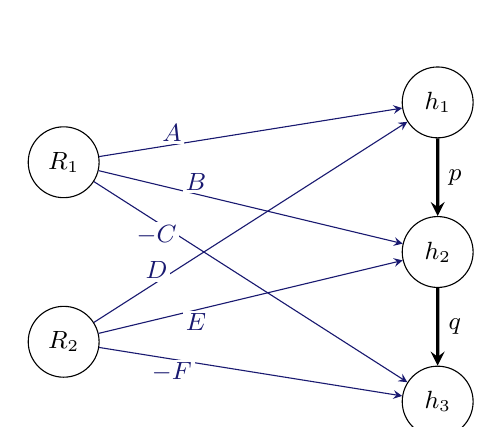
\begin{tikzpicture}[>=stealth,scale=0.95,every node/.style={font=\small}]
\node[draw,circle,minimum size=9mm] (r1) at (0,1.2) {$R_1$};
\node[draw,circle,minimum size=9mm] (r2) at (0,-1.2) {$R_2$};
\node[draw,circle,minimum size=9mm] (h1) at (5,2.0) {$h_1$};
\node[draw,circle,minimum size=9mm] (h2) at (5,0) {$h_2$};
\node[draw,circle,minimum size=9mm] (h3) at (5,-2.0) {$h_3$};
\draw[->,MidnightBlue] (r1) -- node[pos=.24,above,fill=white,inner sep=1pt] {$A$} (h1);
\draw[->,MidnightBlue] (r1) -- node[pos=.32,above,fill=white,inner sep=1pt] {$B$} (h2);
\draw[->,MidnightBlue] (r1) -- node[pos=.20,below,fill=white,inner sep=1pt] {$-C$} (h3);
\draw[->,MidnightBlue] (r2) -- node[pos=.20,above,fill=white,inner sep=1pt] {$D$} (h1);
\draw[->,MidnightBlue] (r2) -- node[pos=.32,below,fill=white,inner sep=1pt] {$E$} (h2);
\draw[->,MidnightBlue] (r2) -- node[pos=.24,below,fill=white,inner sep=1pt] {$-F$} (h3);
\draw[->,very thick] (h1) -- node[right] {$p$} (h2);
\draw[->,very thick] (h2) -- node[right] {$q$} (h3);
\end{tikzpicture}
\caption{Two equations $A+B-C=0$ and $D+E-F=0$ use two common
tree-flow unknowns. Blue edges are prescribed monomials; black edges are free
integer flows. The sum of the squared five vertex divergences, divided by two,
enforces both equations and has unit coefficients before protected substitution.}
\label{fig:two-rows}
\end{figure}

\section{Sharing factors while preserving all coefficients}
\label{sec:aliases}

\subsection{Signed unit normalization}
The source is a finite system $Q_j(x_0,\ldots,x_{n-1})=0$, with each $Q_j$
quadratic and all coefficients integral. The credited predecessor's
normalization is retained. All delivered source variables occur in their
system; unused coordinates may first be removed if only preservation of
existence is needed. Empty residuals may likewise be discarded. Every required
positive coefficient $c>1$ receives
a constant coordinate $C_c$, together with the necessary repeated integer
halves. In increasing order impose
\[
 C_c-2H_c-(c\bmod2)=0,\qquad
 H_c=\begin{cases}1,&\lfloor c/2\rfloor=1,\\
 C_{\lfloor c/2\rfloor},&\lfloor c/2\rfloor>1.
 \end{cases}
\]
Here the coefficient $-2$ is retained as two signed occurrences of $-H_c$.
Every constructor is monic in its new coordinate; thus it forces $C_c=c$.
For each required quadratic coefficient product, introduce a shared scale
$S_{c,i}$ with $S_{c,i}-C_cx_i=0$. Replace $cx_ix_j$ by $S_{c,i}x_j$,
$cx_i$ by $C_cx_i$, and a constant $c$ by $C_c$, retaining signs. This gives
only signed unit occurrences of monomials of degree at most two. All source
solutions extend uniquely to the normalized system, and the inverse is the
projection to the original variables.

This normalization uses binary constructors, not $c$ repeated copies of a term.
The source equation and every monic constructor are retained literally and
checked by exact substitution. No appeal to the numerical size of a hypothetical
solution is involved.

\subsection{Occurrence tags and common factors}
Initially give each signed term occurrence a private coordinate $a_i$.
For a normalized quadratic term $v_jv_k$, choose an orientation and represent
it by $m_i=a_i b_k$, where $a_i$ is an alias of $v_j$ and $b_k$ is a common
representative of $v_k$. All private coordinates, common representatives, and
free graph flows have disjoint names. A linear term $v_j$ is represented by
$a_i u$, where $u$ is one common unit coordinate. A constant term is represented
by $a_i u$ with both coordinates assigned logical value one.

For a square $v_j^2$, the smaller variant uses $m_i=a_i^2$. This changes the
maximum exponent of an individual final coordinate from two to four, but keeps
the total degree four. The variant retaining $a_i b_j$ instead is also valid.

Every ordinary logical variable's aliases are tied together by the cycles below.
All unit aliases, including $u$, are tied to one by a single unit path.
The choice of orientation influences the number of common representatives and
two-element alias groups. The released finite orientation is recorded in the
certificate; its deterministic heuristic is an optimization, not a theorem of
global optimality.

\begin{lemma}[Distinct edge-products with private tags]\label{lem:private}
With distinct private coordinates for each occurrence, the products $m_i^2$
and $m_im_j$ uniquely determine their unordered pair of prescribed occurrences.
Mixed products $m_iw_e$ with free flow coordinates and products of flow
coordinates cannot collide with them or with one another, except for the
intentional commutativity of a product.
\end{lemma}
\begin{proof}
Each prescribed monomial contains its private occurrence coordinate, and no
other prescribed monomial contains that coordinate. Its multiplicity is one
or, for a square occurrence, two. The private part of a pair-product therefore
determines its occurrence multiset. Flow coordinates have a separate namespace.
Prescribed-pair products have degree four, mixed prescribed-flow products degree
three, and flow-pair products degree two. Their namespaces and degrees separate
the three cases.
\end{proof}

\subsection{Reusing factors through a graph without four-cycles}
\label{sec:alias-compression}

The private factor for each term occurrence gives a simple sufficient
condition for coefficient separation. It is stronger than necessary.
We can reuse a private-side alias among occurrences that denote the same
logical first factor, provided a second graph satisfies an elementary
restriction. This \emph{factor graph} is different from the graph whose
divergences define the polynomial.

Put the private-side aliases in one part $A$ and the shared representatives
in another part $S$, including the common unit representative in $S$.
A nonsquare occurrence $m_i=a_is_i$ is an edge between its two factors.
Require that this bipartite graph is simple and has no cycle of length
four. In the version allowing $m_i=a_i^2$, each such square occurrence
keeps an alias that appears in no other source monomial.

\paragraph{Uniqueness of products.}
Suppose that two products of two nonsquare occurrence monomials are equal
as formal monomials. Equality determines the multisets of private-side
and shared-side factors. If either multiset is repeated, simplicity
forces the pair of edges. Otherwise the only possible ambiguity is
\[
 (as)(bt)=(at)(bs), \qquad a\ne b,\quad s\ne t.
\]
The four required edges would form a four-cycle, which is forbidden.
An isolated square occurrence is recognized by its private coordinate,
which occurs in no other source monomial. Products involving such an
occurrence are therefore uniquely recognized as well.

It follows that source-edge squares and products of distinct source
edges never collide after substitution. A source-edge/flow-edge product
is identified by its flow coordinate and its distinct source monomial.
Thus the half-incidence energy still has coefficients in
$\{-1,0,1\}$. The alias equality cycles occupy the separate quadratic
alias namespace, while the flow quadratics use flow coordinates.
The unit path supplies the only linear and constant terms. These
observations establish coefficient separation for the entire polynomial.

\paragraph{Preservation of the zero set.}
An alias is reused only among copies of the same logical normalized
variable. Those copies already agree at every zero of the uncompressed
construction. Conversely, every source zero assigns that logical value
to the reused alias. Rebuild the ordinary equality cycle on the distinct
surviving aliases, adding one dummy exactly when the class has size two.
Both maps on zero sets remain mutually inverse. All internal graph flows
are still uniquely determined by their spanning-tree equations.

\paragraph{A deterministic finite construction.}
The supplied compressor processes occurrences in their recorded order.
It keeps square occurrences separate. An occurrence with shared factor
$s$ can join a private group for the same logical variable if $s$ is new
to the group and no pair $\{s,t\}$ with an existing neighbor $t$ has
already been assigned to another private group. Among eligible groups
it chooses a largest one, with creation order breaking ties. Otherwise
it creates a new group. The neighbor-pair ledger proves inductively that
the factor graph stays simple and has no four-cycle. This is a
deterministic feasible packing, with no assertion of optimality.

On the 442-variable source with 128 hubs and square aliases, this merges
1,969 private occurrences into 1,752 groups. Rebuilding the equality
cycles removes 61 further dummy variables. The resulting complete
polynomial has 2,215 variables and 30,468 monomials, compared with
2,493 variables and 31,186 monomials before this compression. Its total
degree is four, its coefficient height is one, and its individual
variable degrees are at most four. All these counts refer to the fully
collected polynomial, independently reconstructed from the sum of
squares for twice that polynomial.

\subsection{A small example of sharing the flow witnesses}
\label{sec:two-row-example}

Let two abstract residuals be
\[
 R_1=A+B-C,\qquad R_2=D+E-F.
\]
Join their row vertices to three common hub vertices. Only two free
hub-path flows, $p$ and $q$, are needed. The half-incidence energy $\mathcal E$
is specified by
\begin{align*}
 2\mathcal E={}&R_1^2+R_2^2+(p-A-D)^2\\
              &+(q-p-B-E)^2+(C+F-q)^2.
\end{align*}
Every abstract edge symbol occurs in exactly two squared divergences.
Two different edge symbols meet in at most one divergence. Consequently
$\mathcal E$ has integer coefficients of absolute value at most one.
It is nonnegative and vanishes precisely when $R_1=R_2=0$, with the
uniquely determined flows
\[
 p=A+D,\qquad q=A+B+D+E=C+F.
\]
The last equality uses the two residual equations. Away from their
common zero set, choose the polynomial formulas
$p=A+D$ and $q=A+B+D+E$. Then the exact identity is
\[
 \mathcal E=\frac12\bigl(R_1^2+R_2^2+(R_1+R_2)^2\bigr).
\]
This illustrates why sharing hubs preserves the zero set while changing
the off-zero value identity. The general construction substitutes the
protected quadratic occurrence monomials for the six abstract symbols;
the factor-separation argument above prevents coefficient collisions
under that substitution.


\subsection{Equality cycles and the unit path}
For an ordinary logical variable with distinct aliases $a_1,\ldots,a_k$, no
constraint is needed for $k=1$. If $k=2$, append one extra alias. For $k\ge3$ set
\[
 C(a_1,\ldots,a_k)=\sum_{i=1}^k a_i^2-
                         \sum_{i=1}^k a_ia_{i+1},\qquad a_{k+1}=a_1.
\]
Then $2C=\sum_i(a_i-a_{i+1})^2$, so its zeros identify all aliases.
The cycle has length at least three, ensuring every coefficient is $+1$ or $-1$.
A two-cycle would instead create a coefficient $-2$ and is not permitted.

For the unit aliases $u_1,\ldots,u_k$, append fresh coordinates if needed so
that $k\ge2$, and use
\[
 U=1+\sum_{i=1}^k u_i^2-u_1-u_k-
                            \sum_{i=1}^{k-1}u_iu_{i+1}.
\]
The identity
\[
 2U=(u_1-1)^2+\sum_{i=1}^{k-1}(u_i-u_{i+1})^2+(u_k-1)^2
\]
shows that $U\ge0$ and $U=0$ exactly when every unit alias is one. Its two
endpoints are distinct; hence its linear coefficients also have absolute value
one. The graph's quadratic terms involve only flow coordinates, while cycle
and unit-path quadratic terms involve only alias coordinates. No collision
between these components is possible.

\section{The complete compiler theorem}
\label{sec:compiler}

Define the final polynomial by
\begin{equation}\label{eq:wholegraph}
  \boxed{\quad P=\mathcal E_G+\sum_{\text{ordinary alias groups}}C+U.\quad}
\end{equation}
This is a compact mathematical specification of the fully expanded integral
polynomial in the release. All summands are nonnegative at every real point.

\begin{theorem}[Height-one quartic representation]\label{thm:compiler}
For the certified construction above, $P$ is a fixed integer polynomial of
coefficient height one and exact total degree four. Its integer zero set is in
explicit bijection with the integer zero set of the source system $Q_j=0$.
The inverse map is a coordinate projection; the forward map has integer
coefficients and degree at most two.
\end{theorem}
\begin{proof}
The coefficient assertion follows from the simple-graph expansion, the
certified distinctness of prescribed monomial products, and the separate
namespaces for graph and alias constraints. The unit path supplies the sole
constant term, which is one. At least one prescribed edge exists, and its
square is a surviving quartic term; the total degree is therefore exactly four.

Suppose $P=0$ at an integer tuple. Each nonnegative summand must vanish.
The unit path forces every unit alias to one. The equality cycles identify the
aliases of each logical variable. The graph energy forces each divergence to
zero, and summing over a row block recovers that row's normalized equation.
The monic constructors then force their literal constant and scale values,
recovering every original $Q_j=0$.

Conversely, start with a source zero. Compute the constants and scales, assign
every alias its logical value, and assign each prescribed edge its signed
monomial value. Every row balance is zero. Lemma~\ref{lem:tree} assigns the
unique integral free flows that cancel all divergences. All cycles and the unit
path vanish. Thus $P=0$. Constants and scales, aliases, equality dummies, and
tree flows were uniquely assigned, proving the zero-set bijection. Constants
are fixed, scales are linear in source variables, prescribed monomials have
degree at most two, and tree flows are signed sums of those monomials. This
proves the assertion about the degree and integrality of the forward map.
\end{proof}

\subsection{A useful identity away from the zero set}
The forward map can be extended to every source tuple. Root each free tree;
choose flows that cancel all nonroot divergences. The remaining divergence in
row block $r$ is its normalized residual $R_r$, and the hub-root divergence is
$-\sum_rR_r$. The alias constraints still vanish. The normalized constructors
vanish on the canonical extension of the original tuple. Therefore
\begin{equation}\label{eq:offzero}
 P(L(\mathbf x))=\frac12\left(
              \sum_j Q_j(\mathbf x)^2+
                        \left(\sum_jQ_j(\mathbf x)\right)^2\right).
\end{equation}
This is the correct off-zero identity for shared hub vertices. It is generally
different from $\sum_jQ_j^2$. The right side is nevertheless integral and
vanishes exactly when all $Q_j$ vanish. The identity makes no assumption about
the existence of a refutation and gives a useful independent check of the lift.

\subsection{Transferring the consistency interpretation}
The identified source proof gives, in ordinary mathematics formalizable in ZFC,
\[
 \exists\mathbf x\in\Z^n\;\bigwedge_jQ_j(\mathbf x)=0
 \ \longleftrightarrow\
 \text{$\Ctwo$ has the specified finite derivation}
 \ \longleftrightarrow\ \neg\Con(\ZFC).
\]
Theorem~\ref{thm:compiler} is an elementary finite algebraic statement about
integer polynomials, graphs, and trees; its proof is formalizable in ZFC.
Composing the two equivalences and negating proves \eqref{eq:main}. No use of
$\Con(\ZFC)$ as a premise occurs in either direction.

\section{Direct C222 equations with one oriented Pell cap}
\label{sec:direct-cap}
\label{sec:arithmetic}

The direct proof-calculus route now gives two natural quartics and two
integer quartics.  Their coefficients are small enough to be supplied as
complete collected lists.  The integer constructions use a new bounded
congruence that recovers the signs and indices of fifteen Pell pairs at
once.  This section proves the new arithmetic and its composition with
the inherited numerical C222 calculus.  It does not assert a completed
Lean or Rocq derivation.

\begin{center}
\begin{tabular}{lrrrr}
\hline
Domain and variables & Rows & Degree & Terms & Height\\
\hline
$\mathbb N^{240}$ &188&4&25,987&90,589,484\\
$\mathbb N^{239}$ &187&4&360,097&491,869,488\\
$\mathbb Z^{381}$ &225&4&13,179&2,445,790,974,704\\
$\mathbb Z^{391}$ &235&4&10,764&80,496,640\\
\hline
\end{tabular}
\end{center}

Here $\mathbb N=\{0,1,2,\ldots\}$. Each equation is the sum of the
squares of every quadratic residual in its corresponding literal JSON
file. Every declared variable occurs, and the collected single
polynomial has the exact degree and coefficient height shown.  The
240-variable form improves the inspected 261-variable direct natural
form by 21 variables, six rows and 5,692 terms, at a 5.9\% increase in
height. The 381-variable integer form saves 61 variables and 65 rows
against the inspected 442-variable, 290-row direct integer form, but
uses more terms and larger coefficients. These are distinct tradeoffs;
the comparison is confined to the direct C222 architecture.

\subsection{The inherited source and the new composition}

The numerical proof calculus C222 has an inherited, machine-independent
refutation calibration through the named endpoints
\nolinkurl{c222_iff_zf_refutation} and
\nolinkurl{zf_refutation_iff_zfc_refutation}.  The unchanged source
uses beta coding, a nonnegative Horn-flow polynomial, amplified
prime-power CRT, and exact binomial digits.  These complete ordinary
proofs and literal source files are retained in the deliverable.
The new construction does not simulate a K215 execution or instantiate
Jones's universal polynomial.

The incoming shared-binomial construction~\cite{binomial} already uses one binomial
for both a factorial fixed point and a reciprocal CRT product, and
one common Pell residue for eleven binomial numerators.  It retains
six exact power requests but fifteen complete indexed-Pell certificates.
The separate incoming shared-cap construction~\cite{cap} replaces many indexed
certificates by one cap, assuming every requested index belongs to its
power-size frame.  Their combination requires a changed frame: the
modular numerator indices must be included even though their enormous
power outputs are absent.  The compatibility of that enlarged frame
with the cofinal common-root parameter is proved below.

The ordinary source has $t=t_0+16$, a proposed natural factorial $F$,
beta parameters $x,y$, and nine positive encoded CRT representatives.
Set
\[
 B=b_0+2,\quad R=2+t+x+y+F,\quad K=2R,
 \qquad V_0=(F^2+1)^t,\quad N=B^K,\quad q=N^K.
\]
The six exact powers consist of $V_0,N,q$ and
\[
 D_t=q^t,\qquad D_y=q^{y+1},\qquad D_x=q^{x+1}.
\]
The adjacent denominator is the ordinary product
$D_{t+1}=qD_t$.  The one exact binomial digit will identify
$B=\binom{F^2+t}{t}$.  There are ten additional range divisibilities:
the nine independent CRT ranges and the derived-label range.
Every upper index is positive before any power or factorial is
interpreted.  The two raw ceiling rows are
\begin{equation}
 V_0+B=BF+r+1,\qquad B=r+s+1,
 \qquad r,s\in\mathbb N.
 \label{eq:direct-ceiling}
\end{equation}

Let $\mathcal A$ be the set of distinct atoms occurring as bases,
exponents or outputs of the six exact requests, together with the
upper indices of the eleven modular requests.  Its literal size is 23.
The natural construction defines
\begin{equation}
 W=2+\sum_{a\in\mathcal A}a.
 \label{eq:direct-natural-frame}
\end{equation}
Its fifteen distinct requested indices $k_i$ are positive atoms in
$\mathcal A$. Thus $k_i<W$ and $m=15\le W-2$.  No private Pell
coordinate occurs in this definition.

\subsection{A cofinal base above the enlarged frame}

For $a\ge2$, write $(X_j(a),Y_j(a))$ for the Pell sequence defined by
\[
 X_0=1,\ Y_0=0,\qquad
 X_{j+1}=aX_j+(a^2-1)Y_j,\quad Y_{j+1}=X_j+aY_j.
\]
Its elementary properties used below are Pell classification,
strict increase of $Y_j$, and
\[
 X_j(a)\equiv1\pmod{a-1},\qquad
 Y_j(a)\equiv j\pmod{a-1}.
\]
Retain natural witnesses $L,\sigma,Z$ with $Z\ge1$ and
\begin{equation}
 L^2-\bigl((W+1)^2-1\bigr)(WZ)^2=1,
 \qquad A=L+\sigma.
 \label{eq:direct-large-base}
\end{equation}
Pell classification writes $L=X_e(W+1)$ and $WZ=Y_e(W+1)$.
Since $WZ>0$, $e\ge1$; reduction modulo $W$ gives $W\mid e$.
Consequently
\[
 A\ge L\ge X_W(W+1)\ge(W+1)^W.
\]
Conversely $e=W$ supplies $L,Z$, while $A$ remains free to be any
larger integer. This freedom is essential.

Put $b=q+1$ and $M=qD_{t+1}D_xD_y$. The common-root condition is
\begin{equation}
 2Ab=b^2+1+Mh_0.
 \label{eq:direct-common-root}
\end{equation}
For the intended semantic powers, $M$ is a positive power of $q$.
Thus $\gcd(b,M)=1$ and $\gcd(2b,M)\in\{1,2\}$. In the second case
$b$ is odd and $b^2+1$ is even. The linear congruence for $A$ is
soluble, and its solution class has arbitrarily large positive members.
Choose one above $L$ and large enough that $h_0\ge0$. Hence the
enlarged frame and the common root admit simultaneous witnesses.

\subsection{The natural shared cap}

One complete inherited indexed-Pell certificate at index $W$ gives
$V_c=Y_W(A)$. For clarity its polynomial interface is
\begin{align*}
 X_c^2-(A^2-1)V_c^2&=1,& U^2-(A^2-1)V^2&=1,\\
 S^2-(B_c^2-1)T^2&=1,& B_c&=1+4V_c(d+1),\\
 V&=V_c^2(e+1),&B_c&=A+Uf,\\
 S&=X_c+Ug,&T&=W+4V_ch.
\end{align*}
All cap witnesses here are natural. Its usual condition $W\le V_c$
is supplied by the aggregate row below. The indexed-Pell criterion and
its constructive completeness are retained dependencies.

For each of the fifteen other pairs retain only
\[
 x_i^2-(A^2-1)y_i^2=1,
\]
and impose
\begin{equation}
 V_c=W+1+s_c+\sum_i y_i,
 \qquad \sum_i(y_i-k_i)^2=(A-1)Q,
 \quad s_c,Q\in\mathbb N.
 \label{eq:direct-natural-cap}
\end{equation}
Classification gives $y_i=Y_{j_i}(A)$ for $j_i\ge0$.
The first row implies $y_i<V_c$, hence $j_i<W$.
The second implies that $A-1$ divides
$E=\sum_i(j_i-k_i)^2$. But
\[
 0\le E\le m(W-1)^2<W^3<A-1,
\]
so every $j_i=k_i$. This bounds the decoded indices, not the enormous
ordinates.

For completeness choose the canonical pairs. Each $y_i-k_i$ is a
nonnegative multiple of $A-1$. The quotient $Q$ is therefore natural.
Moreover $\sum_i y_i\le mY_{W-1}(A)$ and
$Y_W(A)>(2A-1)Y_{W-1}(A)$. Since $m\le W-2$ and $A>W+1$, the
required slack $s_c=Y_W(A)-W-1-\sum_i y_i$ is nonnegative.

\subsection{The oriented cap over unrestricted integers}

The following is the new sign-removal mechanism. Let $W\ge4$,
$A-1>4W^3$, $1\le k_i<W$, $m\le W-2$, and suppose
$V_c=Y_W(A)$ is already certified. Permit $x_i,y_i,Q$ to be arbitrary
integers, retain their principal norms, and use only
\begin{align}
 V_c&=W+1+s_c+\sum_i y_i^2,&s_c&\in\mathbb N,
 \label{eq:direct-square-cap}\\
 \sum_i\bigl((y_i-k_i)^2+(x_i-1)^2\bigr)&=(A-1)Q.
 \label{eq:direct-oriented-error}
\end{align}
Then
\begin{equation}
 (x_i,y_i)=(X_{k_i}(A),Y_{k_i}(A))
 \quad\text{for every }i.
 \label{eq:direct-oriented-conclusion}
\end{equation}

Indeed signed Pell classification gives
$x_i=\varepsilon_iX_{j_i}(A)$ and
$y_i=\delta_iY_{j_i}(A)$ with independent signs in $\{1,-1\}$.
Equation~\eqref{eq:direct-square-cap} implies $y_i^2<V_c$ and hence
$|y_i|<V_c$, using $|u|\le u^2$ for nonzero integers.
Thus $0\le j_i<W$. Reducing~\eqref{eq:direct-oriented-error}
modulo $A-1$ shows that this modulus divides
\[
 E=\sum_i\bigl((\delta_i j_i-k_i)^2+(\varepsilon_i-1)^2\bigr).
\]
Every summand is nonnegative, and
\[
 0\le E\le m\bigl(4(W-1)^2+4\bigr)<4W^3<A-1.
\]
Therefore $E=0$. It follows that $\varepsilon_i=1$ and
$\delta_i j_i=k_i>0$, proving~\eqref{eq:direct-oriented-conclusion}.
The extra $(x_i-1)^2$ terms are essential for recovering abscissa signs.
There is no sign assumption on the quotient $Q$.

For constructive completeness assume also $2k_i\le W-1$ and $A>W+1$.
Choose all pairs canonical. Their differences $x_i-1$ and $y_i-k_i$
are divisible by $A-1$, so~\eqref{eq:direct-oriented-error} supplies
a natural $Q$. The addition law gives
\[
 Y_{k_i}(A)^2<Y_{2k_i}(A)\le Y_{W-1}(A).
\]
The same recurrence estimate as before makes
$Y_W(A)-\sum_iY_{k_i}(A)^2>W+1$, giving the required natural slack.

The integer source replaces~\eqref{eq:direct-natural-frame} by
\begin{equation}
 W=2+\sum_{a\in\mathcal A}a^2.
 \label{eq:direct-square-frame}
\end{equation}
Even with signed power outputs this bounds every semantic atom in
absolute value by $W$. All fifteen requested indices are positive
before power interpretation, so $m\le W-2$ and
$W\ge k_i^2+2\ge2k_i+1$. The literal $t\ge16$ gives $W\ge258$.
Equation~\eqref{eq:direct-large-base} still yields
\[
 A-1\ge(W+1)^W-1\ge(W+1)^4-1>4W^3.
\]
Thus the square frame proves every hypothesis of the oriented cap.
If zero indices were permitted in a general formulation, a separate
count bound would be needed; they do not occur here.

\subsection{Sequential recovery of power and quotient signs}

After the cap has identified every principal pair, an exact power row is
\begin{equation}
 X_k(A)+(n-A)Y_k(A)=m+T_nu,
 \qquad T_n=2An-n^2-1.
 \label{eq:direct-signed-power}
\end{equation}
Allow $m,u,T_n$ initially to be signed, but suppose $n>0$ is already
known. The square frame gives $1\le n,k<W$ and $|m|<W$.
The polynomial defining $T_n$ is increasing on $1\le n<W$, so
\[
 T_n\ge2A-2>W^W+W,
 \qquad 0<n^k\le(W-1)^{W-1}<W^W.
\]
The usual Pell congruence and~\eqref{eq:direct-signed-power} imply
$T_n\mid m-n^k$. Since $|m-n^k|<T_n$, they force $m=n^k>0$.
The quotient is then nonnegative because the Pell expression is positive
and $m$ is its least positive residue.

The six calls are ordered with bases $F^2+1$, $B$, $N$, and then $q$
three times. The first two are independently positive; their established
outputs license the later bases. The sign argument is consequently
noncircular. It removes the four modulus sign guards and the two output
sign guards that actually remained in the earlier finite census.

The common-root, CRT-index and local-evaluation quotients are needed
only as integer divisibility witnesses for soundness. Their natural signs
follow later from the positive denominators and nonnegative numerators.
The modular-digit quotients are also unrestricted premises: after
recovery the Pell residue is positive and the selected low residue is
least nonnegative, so those quotients are automatically nonnegative.

\subsection{Carry bounds and source calibration}

Equation~\eqref{eq:direct-common-root} gives, for every $n\ge0$,
\[
 X_n(A)+(q+1-A)Y_n(A)\equiv(q+1)^n\pmod M.
\]
This follows by substituting $q+1-A$ for the square root in the Pell
polynomial identity. The resulting expression is positive. Every
required exact-digit modulus $qd$, and every range modulus $Nd$, divides
$M$; the adjacent denominator $D_{t+1}=qD_t$ is included explicitly.
The unchanged remainder rows therefore give the intended digits once
their carry bounds have been established.

The bootstrap is independent of factorial meaning. From $B\ge2$ and
the recovered exact powers, $q\ge2^{4R^2}$. For $0\le j\le t$,
\[
 \binom{F^2+t}{j}\le(F^2+t)^t
 \le(R^2+R)^t\le2^{2Rt}<2^{2R^2}<q.
\]
Thus the exact digit identifies $B=\binom{F^2+t}{t}$.
Equation~\eqref{eq:direct-ceiling} then forces $F>0$ and its inherited
square-radius fixed-point theorem gives $F=t!$.
The retained source proof subsequently establishes every other carry
bound, the reciprocal moduli
$d_i=1+F^2/i$ and their pairwise coprimality, the amplified CRT ranges,
and the finite Horn refutation.  None of these meanings is used before
the preceding power and binomial recovery.

Conversely a finite C222 refutation supplies a padded horizon, its true
factorial, beta parameters, CRT representatives and semantic powers.
Those data determine either enlarged frame before any private Pell
witness. Choose a large compatible $A$ by
\eqref{eq:direct-large-base}--\eqref{eq:direct-common-root}, construct
the one indexed cap and canonical principal pairs, and use the explicit
slacks above. All power and digit quotients then exist. This proves
both directions of the arithmetic source equivalence.

\subsection{Guard graphs, finite identities, and the endpoint}

The integer source retains 52 explicit nonnegativity predicates.
For each selected coordinate $z$, replace its sign condition by the
quadratic row
\[
 z=a^2+b^2+c(c+1),\qquad a,b,c\in\mathbb Z.
\]
This expression is nonnegative and represents every natural number:
apply Legendre's three-square theorem to $4z+1$ and separate the unique
odd square. Every further required sign follows from 174 literal row
consequences, each checked using already known signs or an exact affine
square. The fifteen index-positivity proofs use only the pre-power
source witnesses. The proof never silently treats an exempt signed
coordinate as natural.

The 349-coordinate raw quadratic source with its three changed rows and
52 guard triples has 505 integer variables and 349 residuals. Integral
monic substitution removes 124 coordinates and rows, leaving the stated
381-variable, 225-row quartic. Restricting affine support instead gives
the 391-variable lower-height form. No unconstrained coordinate is
deleted. All inverse substitutions and complete expansions are supplied.

The independent checker imports no source producer, sign-inference
routine or optimizer. It reconstructs the three changed rows, compares
all unchanged rows, checks every guard and sign step, proves the exact
pre-power positivity cut, replays every monic restoration, and compares
every collected quartic coefficient. Separate altered-coefficient and
altered-certificate controls are rejected. These finite checks establish
the emitted arithmetic syntax; the unbounded proof and inherited logic
remain the ordinary arguments just identified.

Negating the resulting equivalence between a polynomial zero and a
finite ZFC refutation gives, for each of the four supplied polynomials,
\[
 \mathrm{ZFC}\ \vdash\
 \bigl(\text{no zero in the stated domain}\bigr)
 \ \longleftrightarrow\ \operatorname{Con}(\mathrm{ZFC}).
\]


\section{A linear strong-Pell multiplier in eleven integers}
\label{sec:linear-multiplier}

This section gives a separate improvement in the small-variable native
construction. It retains the complete source34 coefficient tuple, and hence
its inherited native/compiler/refutation calibration. The new polynomials
have eleven unrestricted integer unknowns. Their exact degree and live
binary-operation counts are
\[
  (440,126)\quad\hbox{and}\quad(412,127).
\]
The newest inspected paired predecessors have profiles $(456,124)$ and
$(416,125)$. The change therefore lowers degree while adding two operations.
It is a new tradeoff, with no assertion of a global minimum. All polynomial
abbreviations below are registers, not additional quantified unknowns.

The idea is to replace the square of the strong Pell multiplier by a linear
input. A coprime product forces that input to become a square at every zero.
Prime-adic orders of polynomial weights keep the radical terms separated, and a
rescaled interpolation request supplies the converse. The sign of the new
input cannot be assumed; recovering it is part of the proof.

\subsection{The literal polynomial}

Let
\[
 j,C,z,h,r,v,w,T,c,n,s\in\mathbb Z.
\]
The six fixed positive coefficients are
$\beta,K_0,M_C,M_F,A_c,B_c$. Their complete integer payloads and finite
reconstruction recipe are supplied with this component. In particular
\[
 \beta=2^{1064921}-1,\qquad A_c=2^{1113},\qquad B_c=2^{666104}.
\]
$M_F$ already includes its source shift. The other three large constants
are the exact whole source34 tuple, not new free parameters.
Define
\begin{align*}
 J&=6j+1,&q&=\beta J+1,&W&=12w+4,\\
 X&=qW,&Y&=qv,&E&=XY,\\
 a&=E+Y,&H&=4a+3,&\Delta&=a^2+H=(a+2)^2-1,\\
 F&=(K_0+W)C-z(q-1),&&&\\
 R&=\bigl(q(q-F)-C\bigr)(q^2-1)+(M_C+qM_F)J,&&&\\
 k&=R+1+hE,&\eta&=c-Yk.&&
\end{align*}
Set
\begin{align*}
 D_{\rm err}&=(A_cF-q)^2+(B_cC-q)^2,\\
 B_{\rm dg}&=k^2(q^2-D_{\rm err})-4q^2\eta^2,\\
 D&=3B_{\rm dg}-4,&\ell&=XY^2,&L&=\ell k,\\
 D_t&=1+L(L+k),&D_g&=1+DD_ts^2,&P&=D_tD_g.
\end{align*}
Here the new multiplier enters linearly:
\begin{align*}
 U&=rc^2,&I_2&=rc^4,&D_f&=1+\Delta I_2,\\
 Q&=\Delta^2I_2,&\delta&=Q-1,&V&=D_f(c-R+4UT)-c,\\
 C_y&=QV^2-1,&D_a&=\delta C_y,&K&=X(3c-2X)+2.
\end{align*}
Finally put
\begin{align*}
 M&=2q^2,&D_c&=MH,&S&=srM^5H,\\
 z_c&=D_cT+MK+H(v-q^2),&&&\\
 A_c^{\ast}&=(z_c^2+3D_c^2)(z_c^3-19D_c^3),&&&\\
 \mathcal A&=9S^2rD_f,&\mathcal B&=S^2D_a,
 &\mathcal G&=81S^2r^2P.
\end{align*}
The starred carrier $A_c^{\ast}$ is unrelated to the fixed cone coefficient
$A_c$. Use $Z=Sn-A_c^{\ast}$ for the direct version and
$Z=S(n+QV)-A_c^{\ast}$ for the centered version. The single equation is
\begin{equation}
 \boxed{\mathcal N=
 \left[(Z^2+\mathcal A-\mathcal B-\mathcal G)^2
       -4(\mathcal AZ^2+\mathcal B\mathcal G)\right]^2
       -64\mathcal AZ^2\mathcal B\mathcal G=0.}
 \label{eq:linear-multiplier-norm}
\end{equation}
The delivered circuits use only integer leaves and binary addition,
subtraction and multiplication. They absorb the fixed scale $81$ into
$D_g$ and reuse $S^2r$. The paired evaluation of the three-root norm is
credited to the incoming Round15 construction. Formally,
\[
 \mathcal N=\prod_{\epsilon\in\{-1,1\}^3}
 \bigl(Z-\epsilon_1\sqrt{\mathcal A}
        -\epsilon_2\sqrt{\mathcal B}
        -\epsilon_3\sqrt{\mathcal G}\bigr).
\]
This is a polynomial identity even when the radicands are dependent,
zero or negative; the radicals are used only in its proof.

\subsection{Signed bootstrap before Pell classification}

The authentic coefficient restrictions give
$q$ even, $q\equiv2\pmod3$, $|q|\ge16$, and $|X|\ge4|q|$.
If $v=0$, then $a=0$ and $\Delta=3$; otherwise $|a|>3$.
Thus $\Delta>1$ on every integer assignment. Also $H$ is odd and
nonzero, $H\equiv3\pmod q$, and $\gcd(H,M)=1$.
Since $X\equiv2\pmod3$, we have $a,H,\Delta\equiv0\pmod3$.
The consecutive product $\ell(\ell+1)$ is nonnegative, so $D_t\ge1$.

The polynomial $\pi(t)=(t^2+3)(t^3-19)$ has no rational root.
Consequently $A_c^{\ast}=D_c^5\pi(z_c/D_c)$ is never zero.
At $S=0$, equation~\eqref{eq:linear-multiplier-norm} reduces to
$(A_c^{\ast})^8=0$, impossible. Every zero therefore has $s,r\ne0$.

The auxiliary radicand $D_a$ is positive without assuming $r>0$.
If $c=0$, then $Q=0$ and $D_a=1$. If $c\ne0,r<0$, then $Q<0$ and
both factors in $(Q-1)(QV^2-1)$ are negative. If $c\ne0,r>0$, then
$Q>1$ and $D_f>|c|+1$. Because $V=D_fb-c$ for an integer $b$, either
$b=0$ and $|V|=|c|\ge1$, or $|V|\ge D_f-|c|>1$; again $D_a>0$.

The product $rD_f$ is nonzero and is positive whenever $c\ne0$.
Its only possible negative case is $c=0,r<0$, when $rD_f=r$.
After dividing a vanishing conjugate factor by $S$, its radical terms,
with independent signs, are
\begin{equation}
 3\sqrt{rD_f},\qquad \sqrt{D_a},\qquad 9r\sqrt P.
 \label{eq:linear-radicals}
\end{equation}
One negative radicand among $rD_f,P$ would leave a single nonzero
imaginary term. If both were negative, cancellation would require
$9(-r)=81r^2(-P)$, hence $1=9rP$, impossible over the integers.
Thus $rD_f>0$ and $P\ge0$. In fact $P>0$: the even fixed cone
coefficients make $B_{\rm dg}$ and $D$ divisible by $4$, so
$D_g\equiv1\pmod4$.

If $B_{\rm dg}\le0$, then $D_g\le-3$, contradicting $P>0$.
Therefore $B_{\rm dg}\ge4$. The usual centered disk inequality yields
$k\ne0$, the common strict sign of $q,F,C,q-F-C$, and
$|c/k-Y|<1/2$. Nonvanishing of $c$ is deferred until the cubic scale
has been recovered.

\subsection{A variable prime-adic separation lemma}

Write $a_3=v_3(|r|)$ and $b_3=v_3(P)$. The congruences
$D_f\equiv D_a\equiv1\pmod3$ imply
$v_3(rD_f)=a_3$ and $v_3(D_a)=0$.
Decompose the positive integer radicands in
\eqref{eq:linear-radicals} into squares times squarefree integers.
For a squareclass whose squarefree part has $3$-adic valuation
$\varepsilon\in\{0,1\}$, the valuations of its coefficients are,
when the corresponding terms occur,
\[
 \begin{array}{c|c}
 \text{auxiliary term}&0\quad(\varepsilon=0\text{ only})\\
 \text{strong term}&1+(a_3-\varepsilon)/2\\
 \text{guard term}&2+a_3+(b_3-\varepsilon)/2.
 \end{array}
\]
If the auxiliary term is present it has uniquely least valuation.
If strong and guard belong to the same class, their valuation difference
is $1+(a_3+b_3)/2>0$. Each nontrivial squareclass therefore has a unique
coefficient of least valuation and cannot cancel. Linear independence
of distinct squarefree radicals forces every radicand in
\eqref{eq:linear-radicals} to be an integer square.

In particular $rD_f$ is a positive square and $\gcd(r,D_f)=1$.
The two factors are either both positive squares or both negatives of
positive squares. The latter would give $-f^2\equiv1\pmod3$, impossible.
Thus
\begin{equation}
 r=u^2>0,\qquad D_f=f^2>0. \label{eq:linear-recovery}
\end{equation}
Also $\gcd(D_t,D_g)=1$ gives $D_t=\tau^2,D_g=g^2$.
The integral radical sum now implies $S\mid A_c^{\ast}$.

Since $M^5\mid S$, monicity of the homogenized quintic gives $M\mid z_c$:
if $p^e\Vert M$ but $v_p(z_c)=b<e$, the leading term $z_c^5$ would have
strictly smaller valuation than every other term of $A_c^{\ast}$.
Reducing modulo $M$ and using $\gcd(M,H)=1$ yields
\[
 v=q^2(2v_{\rm old}+1),\qquad Y=(2v_{\rm old}+1)q^3\ne0.
\]
If $c=0$, the positive budget would equal
$k^2[q^2(1-4Y^2)-D_{\rm err}]\le0$, a contradiction.

Now define the proof-only integer $I=c^2u$. We obtain
\[
 f^2-\Delta I^2=1,\quad Q=(\Delta I)^2>1,\quad
 V=f^2(c-R+4IT_{\rm old})-c,\quad T_{\rm old}=uT.
\]
The rational auxiliary root $\sqrt{D_a}/(Q-1)$ is integral by the
retained adjacent-coefficient Pell descent. Hence the old strong and
auxiliary interfaces, including $c^2\mid I$,
$V\equiv-c\pmod f$ and $V\equiv-R\pmod c$, are all restored.

\subsection{Source recovery and the converse}

The inherited signed rank argument applies to this recovered interface.
It requires neither oddness of $I/c^2$ nor freedom to change
$T_{\rm old}$ at this stage. It gives
\[
 c=\operatorname{sgn}(c)\psi_{a+2}(R),\quad
 R=2t+1,\ t\ge24,\quad
 |Y|>(|X|-3)^t/2-1,\quad |H|>|X|(|X|-3)^t.
\]
The divisibility $H\mid A_c^{\ast}$ gives $H\mid K^5$.
With $\sigma=\operatorname{sgn}(c)$ and
$\Pi=(\sigma X-2^R)(2^R\sigma X+1)$, the retained projection identity
therefore implies $H\mid\Pi^5$. The actual fixed $\beta$ gives
$x=|X|\ge2^{64}$, and
\[
 |\Pi|^5<2^{20t+20}x^{10}<x^{t+1}/2^t<|H|.
\]
The middle inequality follows from $64(t-9)>21t+20$ for $t\ge24$.
Thus $\Pi=0$ and $\sigma X=2^R$. The retained orientation and
centered half-binomial argument restores an actual old native source
zero, and its ordinary calibration yields a finite syntactic refutation.

Conversely, start with the old canonical outer witness supplied by a
finite refutation. It has $D_t=\tau^2$, $B_{\rm dg}\ge64$,
$D_t\equiv1\pmod3$, and $D\equiv2\pmod3$.
Choose a positive Pell solution $g^2-DD_ts^2=1$.
Choose one positive strong pair $I,f$ with $4sc^2\mid I$, and keep it
fixed. Put
\[
 u=I/c^2,\qquad r=u^2,\qquad m=sr=su^2.
\]
The inherited supported-modulus interpolation theorem supplies every
$T_{\rm old}$ residue modulo any positive modulus all of whose prime
divisors divide this fixed $I$. Its full proof is retained in
\texttt{source/POWERED\_PROOF.md}, Section~5.

Canonical projection gives $H\mid K$, so
$\kappa=K/H+(v-q^2)/M$ is integral. Choose an intersective root
$a_0\pmod m$ of $\pi(t+\kappa)$. Every prime divisor of $um=su^3$
divides $I$. Request
\[
 T_{\rm old}\equiv ua_0\pmod{um}.
\]
This yields an auxiliary Pell witness while retaining the same $I,f$.
Consequently $T=T_{\rm old}/u$ is integral and $T\equiv a_0\pmod m$.
Thus
\[
 \frac{A_c^{\ast}}S=\frac{H^4\pi(T+\kappa)}{sr}\in\mathbb Z.
\]
For the direct polynomial take
$n=A_c^{\ast}/S+3uf+\delta y+9r\tau g$; for the centered polynomial
subtract $QV$. One conjugate factor vanishes. The order of witness
choices is outer data, guard pair, fixed strong pair, residue,
auxiliary pair, and finally $n$. The strong pair is never changed after
the residue is requested.

Composing both directions with the retained calibration proves in
ordinary ZFC the equivalence between universal nonvanishing and
$\operatorname{Con}(\mathrm{ZFC})$. This is an ordinary proof composed
with named inherited theorems, not a new complete Lean, Rocq or encoded
object-language ZFC derivation. It proves neither side of that equivalence.

\subsection{Exact degrees and finite validation}

The relevant exact register degrees are
\[
 \begin{array}{c|rrrrrrrrrr}
 \text{register}&I_2&D_f&Q&V&D_a&D_t&P&S&A_c^{\ast}&
       (\mathcal A,\mathcal B,\mathcal G)\\ \hline
 \text{degree}&5&13&21&18&78&22&62&16&35&(46,110,96).
 \end{array}
\]
The direct version has uniquely dominant radicand $\mathcal B$, giving
degree $4\cdot110=440$. In the centered version let $C_0=SQV$ and
$Z_0=Sn-A_c^{\ast}$. The exact defect
\[
 \mathcal B-C_0^2=-S^2\bigl(Q(V^2+1)-1\bigr)
\]
gives $\deg(Z^2-\mathcal B)\le90$.
In the symmetric norm form the inner bracket has unique highest term
$-4\mathcal B\mathcal G$, of degree $206$; its other terms have
degrees at most $192,156,142$. The final correction has degree $362$.
Hence the exact centered degree is $412$.

Let $q_0=6\beta j$, $X_0=12q_0w$, $Y_0=q_0v$,
$R_0=-q_0^3(12wC-q_0z)$ and $k_0=R_0+hX_0Y_0$.
The entire centered highest form is
\[
 2^{64}3^{10}s^{12}r^{20}c^{32}q_0^{84}X_0^{40}Y_0^{52}R_0^4k_0^{12}.
\]
For example the following actual coefficients remain nonzero at the
complete fixed tuple:
\begin{align*}
 [j^{216}w^{52}v^{64}h^{12}z^4s^{12}r^{20}c^{32}]\mathcal N_{
 \rm centered}&=2^{384}3^{278}\beta^{216},\\
 [j^{224}w^{56}v^{56}z^8s^8r^{24}c^{64}]\mathcal N_{
 \rm direct}&=2^{392}3^{280}\beta^{224}.
\end{align*}
These establish exact total degree globally; they are not numerical
samples at particular solutions.

The separate finite checker imports neither the producer nor its DAG
utility. It authenticates the full coefficient tuple and retained source
files, checks all 68 register identities in each circuit over a free
integer polynomial ring, verifies every coefficient of the eight-factor
norm, checks the whole leading forms, and rejects seven changed nodes per
variant. Normal and optimized runs pass, the coefficient recipe reproduces
all six integers byte for byte, and both circuits rebuild identically.
These checks establish finite algebra and transcription claims; the
unbounded Pell and consistency interpretation remain the ordinary proofs
just described.


\section{Exact verification and reproducibility}
\label{sec:verification}
\subsection{Finite checks and ordinary proofs have different jobs}
The graph verifier imports neither graph producer. It checks the literal source
hash, every topological constant/scale constructor and source-row pullback,
the complete logical provenance of every factor, both graph simplicity
conditions, every free spanning tree, and the alias and unit constraints.
It then independently expands the sum of squares for $2P$, divides each even
coefficient by two, and compares every coefficient with the delivered polynomial.
It checks coordinate liveness, total and individual degrees, coefficient height,
the constant term, and all reported counts. Eight concrete corruptions of a
profile must be rejected. The check remains active with Python optimization.

The direct arithmetic checks compare the unchanged inherited source prefix
with its authenticated parent, verify every new semantic row as an exact
polynomial identity, replay the affine export and nonnegative or integer
restoration certificates, and expand the complete sum of squared residuals.
In particular the domain of a removed coordinate is part of a restoration
certificate; a rational identity alone does not justify an integer or
nonnegative-coordinate elimination. The signed cap and sequential recovery
arguments additionally receive ordinary mathematical review.

The eleven-variable branch checks all six actual fixed coefficient payloads,
the literal binary arithmetic graphs, the entire three-radical norm identity,
all new local algebraic identities, and the highest-degree forms at the
authentic coefficient specialization. Its degree statements concern the
whole polynomial, including cancellation, and not only values on its zero set.

The finite checks do not search for a zero, establish that no zero exists,
or use a finite sample as proof of an unbounded Pell or consistency theorem.
The mathematical arguments establishing those implications are supplied in
the report and retained source texts. Recorded review notes state their scope.

\subsection{Reproduction}
The supported entry point is
\begin{quote}\ttfamily
python3 -B verify.py
\end{quote}
from the extracted archive directory. Python's standard library suffices for
the supported new checkers. The runner authenticates the static file manifest
and invokes the component checks with their documented paths. It preserves
the delivered equations. Component receipts record both normal and optimized
checks; the final aggregate receipt records exactly what the release run did.
The component README files document deterministic rebuilds into temporary
directories and their complete byte comparisons. A successful algebraic check
is not labeled a proof-assistant check.

The manuscript builds with a standard TeX Live installation:
\begin{quote}\ttfamily
cd report\\
latexmk -pdf -interaction=nonstopmode -halt-on-error main.tex
\end{quote}
TeX's PDF metadata can vary between builds. Deterministic byte-reproduction
claims concern the polynomial, circuit, and finite-certificate files. The
distributed PDF is itself covered by the release integrity manifest and was
rendered and visually inspected.

\subsection{How to read the literal files}
For a sparse polynomial, a term is written as
\file{[coefficient, [indices]]}. Thus $[-3,[7,7]]$ denotes $-3z_7^2$,
and $[1,[]]$ denotes the constant one. Coordinates are zero-based.
In a residual-system file, the exact final polynomial is the sum of the squares
of every residual, in its printed variable order. An expanded polynomial is
supplied as an additional literal representation. The graph files instead list
their final height-one polynomial directly and carry its half-sum-of-squares
certificate. The eleven-variable files use literal constant, variable, and
binary add/subtract/multiply nodes. A named intermediate node adds no unknown.

The manifest and source hashes detect accidental changes and bind the exact
released data. They do not establish a mathematical theorem by themselves.


\section{What remains open}
\label{sec:future}

\paragraph{A single simplicity objective.}
Variable count, total degree, coefficient height, collected support, and
arithmetic-circuit length are different quantities. There is no proof that one
of the present equations minimizes all of them, or even one globally. A useful
next step is a reproducible Pareto comparison under a fixed domain and complete
coefficient binding, with explicit costs for describing the polynomial.

\paragraph{Better graph layouts.}
The shared-hub family is a transparent constructive choice. Other simple graphs
may reduce $|E_{\rm free}|$ and $\sum_v\binom{\deg v}{2}$ simultaneously.
Free edges must retain an integral completion theorem; arbitrary real linear
dependence would not suffice. More general totally unimodular incidence
structures are a natural direction, provided their collected coefficients stay
controlled.

\paragraph{Better factor sharing.}
The private-tag argument is deliberately strong. Avoiding duplicate pair-products
is the actual requirement. One can study certificate-producing alias packings
under exact multiplicative collision constraints, including how square
occurrences interact with common representatives. Optimizing the number of
normalized terms before allocating aliases is also likely to matter.

\paragraph{Signed arithmetic certificates.}
The arithmetic bottleneck in unrestricted-integer encodings is often sign
recovery, not the number of arithmetic operations in the intended natural
computation. A pooled congruence can recover several signs only after an
independent bound on all possible indices has been established. Preserving this
logical order while sharing the bound further is an explicit research target.

\paragraph{A generic formal proof first.}
The graph compiler has a short proof independent of all inherited Pell and
refutation-calibration theorems. Formalizing its simple-graph, tree-flow, and
monomial-support invariants would provide a reusable verified component.
The source-calibration chain can then be attached with its domain interfaces
visible. This is a more concrete target than treating a successful polynomial
rebuild as an end-to-end formal proof.

\paragraph{Priority and generality.}
The new constructions were compared with the pinned repository and its incoming
archives. A targeted literature search did not establish a prior identical
construction; it also does not establish worldwide priority. The elementary
graph and tree-flow facts are standard linear algebra. The contribution here
is the proved integration, coefficient control, and explicit measured
consistency equations with reproducible finite artifacts.

\appendix
\section{Artifact specification and reading order}
\begin{longtable}{@{}>{\raggedright\arraybackslash}p{.38\textwidth}>{\raggedright\arraybackslash}p{.57\textwidth}@{}}
\toprule
Path & Role\\\midrule\endhead
\file{report/main.tex}, \file{report/main.pdf} & Editable article and its rendered PDF.\\
\file{graph/principal/} & Complete 2,215-variable height-one quartic, plain-text
equation, incidence/factor certificate, and exact metrics.\\
\file{graph/matched519/} & Same-source 2,776-variable height-one comparison,
allowing individual degree four.\\
\file{graph/matched519_no_square/} & Same-source 2,988-variable comparison
retaining individual degree at most two.\\
\file{graph/sources/} & Literal unchanged source442 and source519 residual systems.\\
\file{graph/verify_graph.py}, \file{rebuild.py} & Separate exact checker and
network-free deterministic graph reconstruction.\\
\file{direct/} & New common-cap/modular-binomial arithmetic, literal natural
and signed integer quartics, semantic and restoration certificates, ordinary
proofs, and independent finite checks.\\
\file{low_variable/} & New eleven-integer polynomial circuits, fixed
coefficient payloads and reconstruction recipe, complete new proof, and checks.\\
\file{inherited/} & Selected unchanged source proofs, calibration interfaces,
licenses, and original notices.\\
\file{provenance/} & Frozen repository and archive identities, and maps between
original source members and retained local files.\\
\file{reviews/} & Separately tasked mathematical reviews and their exact scope.\\
\file{MANIFEST.json}, \file{RELEASE.json} & Static integrity inventory and
machine-readable released equation claims.\\
\bottomrule
\end{longtable}

For the graph result, read Sections~\ref{sec:graph}--\ref{sec:compiler}, then
the literal polynomial and its independently verified certificate. For the
consistency interpretation, read the source442 ordinary signed source proof,
its unified binomial/CRT dependencies, and the C222/ZF/ZFC interfaces identified
in the source ledger. For the arithmetic improvements, read the new proof
before consulting finite test receipts. The latter support exact algebraic and
artifact claims and do not replace the unbounded arguments.


\section{Source provenance and calibration}
The public snapshot is pinned by its full Git commit, not by a moving branch
name. All eight downloaded incoming archives were checked against their Git
blob SHA-1 identifiers as well as recorded SHA-256 hashes and byte counts.
\file{provenance/REPOSITORY_SNAPSHOT.json} records this acquisition boundary.
It is a provenance check, not a mathematical proof or an authenticated signature.

The graph branch's two literal source systems are preserved unchanged in
\file{graph/sources/source442.json} and \file{graph/sources/source519.json}.
Their original archive members and byte hashes are recorded with them.
The calibrated source systems have unrestricted integer coordinates. The
transformations in this report do not infer a sign restriction for an
unrestricted coordinate merely from its intended computational meaning.

The retained source collection includes the earlier proof/calibration reading
packet, the later selectively-even-index and unified-product arguments, and
their arithmetic proof dependencies. Byte-identical copies already supplied
by another component are shared rather than duplicated. The copied texts
remain unchanged; their original archive-member paths and exact current local
filenames are listed in \file{provenance/INHERITED_SOURCES.json}. Five redundant
historical repository overviews are recorded by provenance rather than copied.
Every mathematical dependency selected for this collection is retained. Some
historical relative links refer to the original packet; the ledger is the
authoritative map in this release. These retained texts are mathematical
dependencies, not new claims of authorship or new formal-kernel certificates.

The generic graph normalization is adapted from the incoming height-one
compiler; the equality-cycle and unit-path gadgets are credited to that
packet. The shared incidence graph, common factor representatives, certified
four-cycle-free factor reuse, measured equations, and their new independent
checks are the contributions of the present graph branch.

The direct arithmetic branch has its own retained source map and notices.
The new source takes the modular binomial arithmetic from one incoming packet
and the common Pell cap from another. Their compatibility is proved here by
rebuilding all private witnesses after enlarging the semantic frame; it is
not inferred from the separate satisfiability of the two predecessor systems.

The source-calibration development includes proof-assistant interface files.
Reading those files identifies the theorem statements used. This release does
not claim to rebuild their full transitive import closure or export a formal
ZFC proof object. The new unbounded arguments are ordinary proofs; the scripts
are exact finite algebraic and artifact checks. Neither kind of evidence is
represented as the other.

All new research, code, and exposition in this packet were prepared with AI
assistance. Separate research-agent reviews are internal checks within this
workflow, not external human peer review or institutional endorsement.
Original source licenses and notices are retained, and new material is offered
under the repository's MIT No Attribution terms.


\section{Literal residuals of the 381-integer quartic}
\label{app:integer381-residuals}
All coordinates $z_0,\ldots,z_{380}$ range over $\mathbb Z$. The equation is
\[P_{381}(z)=\sum_{j=0}^{224}R_j(z)^2=0.\]
The following list contains every residual, in the authoritative JSON order.
\begingroup\small\allowdisplaybreaks
\begin{align*}
R_{0} &= -z_{3}^{2} +z_{4} \\
R_{1} &= 1 -2z_{3} -z_{3}z_{5} +z_{5} \\
&\quad +z_{6} -z_{234}^{2} -z_{235}^{2} -z_{236} \\
&\quad -z_{236}^{2} \\
R_{2} &= -z_{0}z_{2} -17z_{2} +z_{9} \\
R_{3} &= -1 +z_{1} -z_{2}z_{7} -z_{3} \\
&\quad -z_{7} \\
R_{4} &= -1 +z_{1} -z_{8} -z_{8}z_{9} \\
R_{5} &= 2 +z_{4} -z_{5}z_{20} +z_{18} \\
&\quad -2z_{20} \\
R_{6} &= -6 -5z_{10} -z_{10}^{2} -2z_{10}z_{11} \\
&\quad -5z_{11} -z_{11}^{2} +z_{21} \\
R_{7} &= -72 -68z_{11} -16z_{11}^{2} -16z_{11}z_{21} \\
&\quad -34z_{21} -4z_{21}^{2} +z_{22} \\
R_{8} &= -30 -11z_{10} -z_{10}^{2} -4z_{10}z_{22} \\
&\quad -22z_{22} -4z_{22}^{2} +z_{23} \\
R_{9} &= -380 -312z_{22} -64z_{22}^{2} -32z_{22}z_{23} \\
&\quad -78z_{23} -4z_{23}^{2} +z_{24} \\
R_{10} &= -6 -5z_{11} -z_{11}^{2} -2z_{11}z_{12} \\
&\quad -5z_{12} -z_{12}^{2} +z_{25} \\
R_{11} &= -30 -11z_{10} -z_{10}^{2} -8z_{10}z_{12} \\
&\quad -4z_{10}z_{25} -44z_{12} -16z_{12}^{2} -16z_{12}z_{25} \\
&\quad -22z_{25} -4z_{25}^{2} +z_{26} \\
R_{12} &= -6 -5z_{10} -z_{10}^{2} -2z_{10}z_{12} \\
&\quad -5z_{12} -z_{12}^{2} +z_{27} \\
R_{13} &= -156 -100z_{11} -16z_{11}^{2} -32z_{11}z_{12} \\
&\quad -16z_{11}z_{21} -16z_{11}z_{27} -100z_{12} -16z_{12}^{2} \\
&\quad -16z_{12}z_{21} -16z_{12}z_{27} -50z_{21} -4z_{21}^{2} \\
&\quad -8z_{21}z_{27} -50z_{27} -4z_{27}^{2} +z_{28} \\
R_{14} &= -1806 -2720z_{12} -1024z_{12}^{2} -512z_{12}z_{25} \\
&\quad -128z_{12}z_{26} -512z_{12}z_{27} -128z_{12}z_{28} -680z_{25} \\
&\quad -64z_{25}^{2} -32z_{25}z_{26} -128z_{25}z_{27} -32z_{25}z_{28} \\
&\quad -170z_{26} -4z_{26}^{2} -32z_{26}z_{27} -8z_{26}z_{28} \\
&\quad -680z_{27} -64z_{27}^{2} -32z_{27}z_{28} -170z_{28} \\
&\quad -4z_{28}^{2} +z_{29} \\
R_{15} &= -110 -84z_{10} -16z_{10}^{2} -32z_{10}z_{11} \\
&\quad -16z_{10}z_{25} -16z_{10}z_{27} -84z_{11} -16z_{11}^{2} \\
&\quad -16z_{11}z_{25} -16z_{11}z_{27} -42z_{25} -4z_{25}^{2} \\
&\quad -8z_{25}z_{27} -42z_{27} -4z_{27}^{2} +z_{30} \\
R_{16} &= -756 -1100z_{11} -400z_{11}^{2} -80z_{11}z_{21} \\
&\quad -320z_{11}z_{25} -80z_{11}z_{30} -110z_{21} -4z_{21}^{2} \\
&\quad -32z_{21}z_{25} -8z_{21}z_{30} -440z_{25} -64z_{25}^{2} \\
&\quad -32z_{25}z_{30} -110z_{30} -4z_{30}^{2} +z_{31} \\
R_{17} &= -56 -15z_{10} -z_{10}^{2} -8z_{10}z_{12} \\
&\quad -4z_{10}z_{25} -60z_{12} -16z_{12}^{2} -16z_{12}z_{25} \\
&\quad -30z_{25} -4z_{25}^{2} +z_{32} \\
R_{18} &= -56 -15z_{11} -z_{11}^{2} -8z_{11}z_{12} \\
&\quad -4z_{11}z_{27} -60z_{12} -16z_{12}^{2} -16z_{12}z_{27} \\
&\quad -30z_{27} -4z_{27}^{2} +z_{33} \\
R_{19} &= -2756 -3360z_{12} -1024z_{12}^{2} -512z_{12}z_{25} \\
&\quad -512z_{12}z_{27} -128z_{12}z_{32} -128z_{12}z_{33} -840z_{25} \\
&\quad -64z_{25}^{2} -128z_{25}z_{27} -32z_{25}z_{32} -32z_{25}z_{33} \\
&\quad -840z_{27} -64z_{27}^{2} -32z_{27}z_{32} -32z_{27}z_{33} \\
&\quad -210z_{32} -4z_{32}^{2} -8z_{32}z_{33} -210z_{33} \\
&\quad -4z_{33}^{2} +z_{34} \\
R_{20} &= -110 -168z_{11} -64z_{11}^{2} -32z_{11}z_{21} \\
&\quad -32z_{11}z_{25} -42z_{21} -4z_{21}^{2} -8z_{21}z_{25} \\
&\quad -42z_{25} -4z_{25}^{2} +z_{35} \\
R_{21} &= -756 -220z_{10} -16z_{10}^{2} -128z_{10}z_{11} \\
&\quad -64z_{10}z_{21} -16z_{10}z_{27} -16z_{10}z_{35} -880z_{11} \\
&\quad -256z_{11}^{2} -256z_{11}z_{21} -64z_{11}z_{27} -64z_{11}z_{35} \\
&\quad -440z_{21} -64z_{21}^{2} -32z_{21}z_{27} -32z_{21}z_{35} \\
&\quad -110z_{27} -4z_{27}^{2} -8z_{27}z_{35} -110z_{35} \\
&\quad -4z_{35}^{2} +z_{36} \\
R_{22} &= -56 -60z_{11} -16z_{11}^{2} -16z_{11}z_{21} \\
&\quad -30z_{21} -4z_{21}^{2} +z_{37} \\
R_{23} &= -30 -11z_{10} -z_{10}^{2} -4z_{10}z_{37} \\
&\quad -22z_{37} -4z_{37}^{2} +z_{38} \\
R_{24} &= -380 -312z_{37} -64z_{37}^{2} -32z_{37}z_{38} \\
&\quad -78z_{38} -4z_{38}^{2} +z_{39} \\
R_{25} &= -30 -11z_{11} -z_{11}^{2} -4z_{11}z_{39} \\
&\quad -22z_{39} -4z_{39}^{2} +z_{40} \\
R_{26} &= -156 -200z_{11} -64z_{11}^{2} -64z_{11}z_{21} \\
&\quad -100z_{21} -16z_{21}^{2} +z_{41} \\
R_{27} &= -1406 -1500z_{11} -400z_{11}^{2} -320z_{11}z_{21} \\
&\quad -80z_{11}z_{25} -80z_{11}z_{41} -600z_{21} -64z_{21}^{2} \\
&\quad -32z_{21}z_{25} -32z_{21}z_{41} -150z_{25} -4z_{25}^{2} \\
&\quad -8z_{25}z_{41} -150z_{41} -4z_{41}^{2} +z_{42} \\
R_{28} &= -16256 -1020z_{10} -16z_{10}^{2} -512z_{10}z_{11} \\
&\quad -256z_{10}z_{21} -16z_{10}z_{27} -64z_{10}z_{41} -16z_{10}z_{42} \\
&\quad -16320z_{11} -4096z_{11}^{2} -4096z_{11}z_{21} -256z_{11}z_{27} \\
&\quad -1024z_{11}z_{41} -256z_{11}z_{42} -8160z_{21} -1024z_{21}^{2} \\
&\quad -128z_{21}z_{27} -512z_{21}z_{41} -128z_{21}z_{42} -510z_{27} \\
&\quad -4z_{27}^{2} -32z_{27}z_{41} -8z_{27}z_{42} -2040z_{41} \\
&\quad -64z_{41}^{2} -32z_{41}z_{42} -510z_{42} -4z_{42}^{2} \\
&\quad +z_{43} \\
R_{29} &= -6 -5z_{12} -z_{12}^{2} -2z_{12}z_{13} \\
&\quad -5z_{13} -z_{13}^{2} +z_{44} \\
R_{30} &= -30 -11z_{10} -z_{10}^{2} -8z_{10}z_{13} \\
&\quad -4z_{10}z_{44} -44z_{13} -16z_{13}^{2} -16z_{13}z_{44} \\
&\quad -22z_{44} -4z_{44}^{2} +z_{45} \\
R_{31} &= -72 -136z_{12} -64z_{12}^{2} -32z_{12}z_{25} \\
&\quad -32z_{12}z_{27} -34z_{25} -4z_{25}^{2} -8z_{25}z_{27} \\
&\quad -34z_{27} -4z_{27}^{2} +z_{46} \\
R_{32} &= -420 -164z_{10} -16z_{10}^{2} -128z_{10}z_{12} \\
&\quad -64z_{10}z_{25} -16z_{10}z_{45} -16z_{10}z_{46} -656z_{12} \\
&\quad -256z_{12}^{2} -256z_{12}z_{25} -64z_{12}z_{45} -64z_{12}z_{46} \\
&\quad -328z_{25} -64z_{25}^{2} -32z_{25}z_{45} -32z_{25}z_{46} \\
&\quad -82z_{45} -4z_{45}^{2} -8z_{45}z_{46} -82z_{46} \\
&\quad -4z_{46}^{2} +z_{47} \\
R_{33} &= -462 -688z_{11} -256z_{11}^{2} -32z_{11}z_{12} \\
&\quad -256z_{11}z_{25} -64z_{11}z_{30} -43z_{12} -z_{12}^{2} \\
&\quad -16z_{12}z_{25} -4z_{12}z_{30} -344z_{25} -64z_{25}^{2} \\
&\quad -32z_{25}z_{30} -86z_{30} -4z_{30}^{2} +z_{48} \\
R_{34} &= -42 -52z_{12} -16z_{12}^{2} -16z_{12}z_{25} \\
&\quad -26z_{25} -4z_{25}^{2} +z_{49} \\
R_{35} &= -30 -11z_{12} -z_{12}^{2} -4z_{12}z_{49} \\
&\quad -22z_{49} -4z_{49}^{2} +z_{50} \\
R_{36} &= -306 -35z_{11} -z_{11}^{2} -16z_{11}z_{49} \\
&\quad -4z_{11}z_{50} -280z_{49} -64z_{49}^{2} -32z_{49}z_{50} \\
&\quad -70z_{50} -4z_{50}^{2} +z_{51} \\
R_{37} &= -4556 -4320z_{49} -1024z_{49}^{2} -512z_{49}z_{50} \\
&\quad -128z_{49}z_{51} -1080z_{50} -64z_{50}^{2} -32z_{50}z_{51} \\
&\quad -270z_{51} -4z_{51}^{2} +z_{52} \\
R_{38} &= -30 -11z_{12} -z_{12}^{2} -4z_{12}z_{52} \\
&\quad -22z_{52} -4z_{52}^{2} +z_{53} \\
R_{39} &= -306 -35z_{11} -z_{11}^{2} -16z_{11}z_{52} \\
&\quad -4z_{11}z_{53} -280z_{52} -64z_{52}^{2} -32z_{52}z_{53} \\
&\quad -70z_{53} -4z_{53}^{2} +z_{54} \\
R_{40} &= -22052 -19008z_{11} -4096z_{11}^{2} -4096z_{11}z_{25} \\
&\quad -1024z_{11}z_{30} -256z_{11}z_{48} -4096z_{11}z_{52} -1024z_{11}z_{53} \\
&\quad -256z_{11}z_{54} -9504z_{25} -1024z_{25}^{2} -512z_{25}z_{30} \\
&\quad -128z_{25}z_{48} -2048z_{25}z_{52} -512z_{25}z_{53} -128z_{25}z_{54} \\
&\quad -2376z_{30} -64z_{30}^{2} -32z_{30}z_{48} -512z_{30}z_{52} \\
&\quad -128z_{30}z_{53} -32z_{30}z_{54} -594z_{48} -4z_{48}^{2} \\
&\quad -128z_{48}z_{52} -32z_{48}z_{53} -8z_{48}z_{54} -9504z_{52} \\
&\quad -1024z_{52}^{2} -512z_{52}z_{53} -128z_{52}z_{54} -2376z_{53} \\
&\quad -64z_{53}^{2} -32z_{53}z_{54} -594z_{54} -4z_{54}^{2} \\
&\quad +z_{55} \\
R_{41} &= -70490 -531z_{10} -z_{10}^{2} -256z_{10}z_{52} \\
&\quad -64z_{10}z_{53} -16z_{10}z_{54} -4z_{10}z_{55} -67968z_{52} \\
&\quad -16384z_{52}^{2} -8192z_{52}z_{53} -2048z_{52}z_{54} -512z_{52}z_{55} \\
&\quad -16992z_{53} -1024z_{53}^{2} -512z_{53}z_{54} -128z_{53}z_{55} \\
&\quad -4248z_{54} -64z_{54}^{2} -32z_{54}z_{55} -1062z_{55} \\
&\quad -4z_{55}^{2} +z_{56} \\
R_{42} &= -1122540 -1084928z_{52} -262144z_{52}^{2} -131072z_{52}z_{53} \\
&\quad -32768z_{52}z_{54} -8192z_{52}z_{55} -2048z_{52}z_{56} -271232z_{53} \\
&\quad -16384z_{53}^{2} -8192z_{53}z_{54} -2048z_{53}z_{55} -512z_{53}z_{56} \\
&\quad -67808z_{54} -1024z_{54}^{2} -512z_{54}z_{55} -128z_{54}z_{56} \\
&\quad -16952z_{55} -64z_{55}^{2} -32z_{55}z_{56} -4238z_{56} \\
&\quad -4z_{56}^{2} +z_{57} \\
R_{43} &= -30 -11z_{12} -z_{12}^{2} -4z_{12}z_{57} \\
&\quad -22z_{57} -4z_{57}^{2} +z_{58} \\
R_{44} &= -306 -35z_{10} -z_{10}^{2} -16z_{10}z_{57} \\
&\quad -4z_{10}z_{58} -280z_{57} -64z_{57}^{2} -32z_{57}z_{58} \\
&\quad -70z_{58} -4z_{58}^{2} +z_{59} \\
R_{45} &= -4556 -4320z_{57} -1024z_{57}^{2} -512z_{57}z_{58} \\
&\quad -128z_{57}z_{59} -1080z_{58} -64z_{58}^{2} -32z_{58}z_{59} \\
&\quad -270z_{59} -4z_{59}^{2} +z_{60} \\
R_{46} &= -90 -76z_{12} -16z_{12}^{2} -16z_{12}z_{25} \\
&\quad -16z_{12}z_{60} -38z_{25} -4z_{25}^{2} -8z_{25}z_{60} \\
&\quad -38z_{60} -4z_{60}^{2} +z_{61} \\
R_{47} &= -306 -35z_{11} -z_{11}^{2} -16z_{11}z_{60} \\
&\quad -4z_{11}z_{61} -280z_{60} -64z_{60}^{2} -32z_{60}z_{61} \\
&\quad -70z_{61} -4z_{61}^{2} +z_{62} \\
R_{48} &= -4556 -4320z_{52} -1024z_{52}^{2} -512z_{52}z_{53} \\
&\quad -128z_{52}z_{54} -1080z_{53} -64z_{53}^{2} -32z_{53}z_{54} \\
&\quad -270z_{54} -4z_{54}^{2} +z_{63} \\
R_{49} &= -4970 -4512z_{60} -1024z_{60}^{2} -512z_{60}z_{61} \\
&\quad -128z_{60}z_{62} -128z_{60}z_{63} -1128z_{61} -64z_{61}^{2} \\
&\quad -32z_{61}z_{62} -32z_{61}z_{63} -282z_{62} -4z_{62}^{2} \\
&\quad -8z_{62}z_{63} -282z_{63} -4z_{63}^{2} +z_{64} \\
R_{50} &= -306 -35z_{12} -z_{12}^{2} -16z_{12}z_{63} \\
&\quad -4z_{12}z_{64} -280z_{63} -64z_{63}^{2} -32z_{63}z_{64} \\
&\quad -70z_{64} -4z_{64}^{2} +z_{65} \\
R_{51} &= -42 -52z_{11} -16z_{11}^{2} -8z_{11}z_{12} \\
&\quad -16z_{11}z_{21} -13z_{12} -z_{12}^{2} -4z_{12}z_{21} \\
&\quad -26z_{21} -4z_{21}^{2} +z_{66} \\
R_{52} &= -756 -1100z_{11} -400z_{11}^{2} -400z_{11}z_{21} \\
&\quad -80z_{11}z_{66} -550z_{21} -100z_{21}^{2} -40z_{21}z_{66} \\
&\quad -110z_{66} -4z_{66}^{2} +z_{67} \\
R_{53} &= -23870 -19776z_{11} -4096z_{11}^{2} -4096z_{11}z_{21} \\
&\quad -4096z_{11}z_{63} -1024z_{11}z_{64} -256z_{11}z_{65} -1024z_{11}z_{66} \\
&\quad -256z_{11}z_{67} -9888z_{21} -1024z_{21}^{2} -2048z_{21}z_{63} \\
&\quad -512z_{21}z_{64} -128z_{21}z_{65} -512z_{21}z_{66} -128z_{21}z_{67} \\
&\quad -9888z_{63} -1024z_{63}^{2} -512z_{63}z_{64} -128z_{63}z_{65} \\
&\quad -512z_{63}z_{66} -128z_{63}z_{67} -2472z_{64} -64z_{64}^{2} \\
&\quad -32z_{64}z_{65} -128z_{64}z_{66} -32z_{64}z_{67} -618z_{65} \\
&\quad -4z_{65}^{2} -32z_{65}z_{66} -8z_{65}z_{67} -2472z_{66} \\
&\quad -64z_{66}^{2} -32z_{66}z_{67} -618z_{67} -4z_{67}^{2} \\
&\quad +z_{68} \\
R_{54} &= -70490 -67968z_{63} -16384z_{63}^{2} -8192z_{63}z_{64} \\
&\quad -2048z_{63}z_{65} -512z_{63}z_{68} -16992z_{64} -1024z_{64}^{2} \\
&\quad -512z_{64}z_{65} -128z_{64}z_{68} -4248z_{65} -64z_{65}^{2} \\
&\quad -32z_{65}z_{68} -1062z_{68} -4z_{68}^{2} +z_{69} \\
R_{55} &= -z_{3} -z_{3}z_{15} +z_{70} \\
R_{56} &= -z_{14}^{2} +2z_{14}z_{15} -z_{15}^{2} +z_{71} \\
R_{57} &= -2z_{24}z_{70} -4z_{70} +z_{72} \\
R_{58} &= -z_{14}^{2} +2z_{14}z_{15} +2z_{14}z_{72} -z_{15}^{2} \\
&\quad -2z_{15}z_{72} -z_{72}^{2} +z_{73} \\
R_{59} &= -64z_{12}z_{70} -32z_{27}z_{70} -8z_{28}z_{70} -2z_{29}z_{70} \\
&\quad -96z_{70} +z_{74} \\
R_{60} &= -z_{14}^{2} +2z_{14}z_{15} +2z_{14}z_{74} -z_{15}^{2} \\
&\quad -2z_{15}z_{74} -z_{74}^{2} +z_{75} \\
R_{61} &= -64z_{11}z_{70} -32z_{25}z_{70} -8z_{30}z_{70} -2z_{31}z_{70} \\
&\quad -80z_{70} +z_{76} \\
R_{62} &= -z_{14}^{2} +2z_{14}z_{15} +2z_{14}z_{76} -z_{15}^{2} \\
&\quad -2z_{15}z_{76} -z_{76}^{2} +z_{77} \\
R_{63} &= -64z_{12}z_{70} -32z_{27}z_{70} -8z_{33}z_{70} -2z_{34}z_{70} \\
&\quad -104z_{70} +z_{78} \\
R_{64} &= -z_{14}^{2} +2z_{14}z_{15} +2z_{14}z_{78} -z_{15}^{2} \\
&\quad -2z_{15}z_{78} -z_{78}^{2} +z_{79} \\
R_{65} &= -64z_{11}z_{70} -32z_{21}z_{70} -8z_{35}z_{70} -2z_{36}z_{70} \\
&\quad -80z_{70} +z_{80} \\
R_{66} &= -z_{14}^{2} +2z_{14}z_{15} +2z_{14}z_{80} -z_{15}^{2} \\
&\quad -2z_{15}z_{80} -z_{80}^{2} +z_{81} \\
R_{67} &= -4z_{11}z_{70} -2z_{40}z_{70} -4z_{70} +z_{82} \\
R_{68} &= -z_{14}^{2} +2z_{14}z_{15} +2z_{14}z_{82} -z_{15}^{2} \\
&\quad -2z_{15}z_{82} -z_{82}^{2} +z_{83} \\
R_{69} &= -256z_{11}z_{70} -128z_{21}z_{70} -32z_{41}z_{70} -8z_{42}z_{70} \\
&\quad -2z_{43}z_{70} -480z_{70} +z_{84} \\
R_{70} &= -z_{14}^{2} +2z_{14}z_{15} +2z_{14}z_{84} -z_{15}^{2} \\
&\quad -2z_{15}z_{84} -z_{84}^{2} +z_{85} \\
R_{71} &= -64z_{12}z_{70} -32z_{25}z_{70} -8z_{46}z_{70} -2z_{47}z_{70} \\
&\quad -64z_{70} +z_{86} \\
R_{72} &= -z_{14}^{2} +2z_{14}z_{15} +2z_{14}z_{86} -z_{15}^{2} \\
&\quad -2z_{15}z_{86} -z_{86}^{2} +z_{87} \\
R_{73} &= -z_{10}^{2} +2z_{10}z_{12} -z_{12}^{2} +z_{88} \\
R_{74} &= -z_{11}^{2} +2z_{11}z_{12} -z_{12}^{2} +z_{89} \\
R_{75} &= -z_{88}z_{89} +z_{90} \\
R_{76} &= -4 -4z_{13} -z_{13}^{2} +z_{91} \\
R_{77} &= -z_{90}^{2} +2z_{90}z_{91} -z_{91}^{2} +z_{92} \\
R_{78} &= -2z_{69}z_{70} -4z_{70} +z_{93} \\
R_{79} &= -z_{14}^{2} +2z_{14}z_{15} +2z_{14}z_{93} -z_{15}^{2} \\
&\quad -2z_{15}z_{93} -z_{93}^{2} +z_{94} \\
R_{80} &= -z_{3} -z_{3}z_{11} +z_{95} \\
R_{81} &= -1 -z_{15} -z_{15}z_{95} -z_{95} \\
&\quad +z_{96} \\
R_{82} &= -z_{3} -z_{3}z_{10} +z_{97} \\
R_{83} &= -4z_{3} -4z_{3}z_{11} -2z_{3}z_{21} +z_{98} \\
R_{84} &= -1 -z_{14} -z_{14}z_{97} -z_{97} \\
&\quad +z_{99} \\
R_{85} &= -z_{98}z_{99} -z_{99} +z_{100} \\
R_{86} &= -z_{96}^{2} +2z_{96}z_{100} -z_{100}^{2} +z_{101} \\
R_{87} &= -6z_{3} -4z_{3}z_{11} -2z_{3}z_{21} +z_{102} \\
R_{88} &= -1 -z_{15} -z_{15}z_{102} -z_{102} \\
&\quad +z_{103} \\
R_{89} &= -1 -z_{14} -z_{14}z_{95} -z_{95} \\
&\quad +z_{104} \\
R_{90} &= -z_{103}^{2} +2z_{103}z_{104} -z_{104}^{2} +z_{105} \\
R_{91} &= -z_{71}z_{73} +z_{106} \\
R_{92} &= -z_{75}z_{106} +z_{107} \\
R_{93} &= -z_{77}z_{107} +z_{108} \\
R_{94} &= -z_{79}z_{108} +z_{109} \\
R_{95} &= -z_{81}z_{109} +z_{110} \\
R_{96} &= -z_{83}z_{110} +z_{111} \\
R_{97} &= -z_{85}z_{111} +z_{112} \\
R_{98} &= -z_{87}z_{112} +z_{113} \\
R_{99} &= -z_{92}z_{113} -z_{94}z_{113} +z_{114} \\
R_{100} &= -z_{101}z_{114} +z_{115} \\
R_{101} &= -2z_{2} -z_{2}z_{18} +z_{116} \\
R_{102} &= -1 -z_{16} -z_{16}z_{116} -z_{116} \\
&\quad +z_{117} \\
R_{103} &= -2 +4z_{1} -2z_{1}^{2} +2z_{1}z_{14} \\
&\quad +2z_{1}z_{15} +2z_{1}z_{117} +2z_{1}z_{118} -2z_{14} \\
&\quad -z_{14}^{2} -2z_{14}z_{117} -2z_{15} -z_{15}^{2} \\
&\quad -2z_{15}z_{118} +z_{19}z_{120} -z_{105}z_{115} -2z_{117} \\
&\quad -z_{117}^{2} -2z_{118} -z_{118}^{2} \\
R_{104} &= -1 -z_{2} -z_{2}z_{17} -z_{17} \\
&\quad -z_{17}z_{116} -z_{116} +z_{118} \\
R_{105} &= -922 -z_{10} -393z_{11} -192z_{12} \\
&\quad -162z_{21} -2z_{24} -64z_{25} -64z_{27} \\
&\quad -8z_{28} -2z_{29} -8z_{30} -2z_{31} \\
&\quad -8z_{33} -2z_{34} -8z_{35} -2z_{36} \\
&\quad -2z_{40} -32z_{41} -8z_{42} -2z_{43} \\
&\quad -8z_{46} -2z_{47} -2z_{69} +z_{119} \\
R_{106} &= 1 -z_{121}z_{122} +z_{181} +z_{182} \\
R_{107} &= -z_{121} -z_{121}z_{181} -z_{121}z_{182} +z_{125} \\
R_{108} &= -z_{123}z_{125} +z_{126} \\
R_{109} &= -z_{124}z_{126} +z_{127} \\
R_{110} &= -z_{128} -z_{128}z_{131} +z_{132} \\
R_{111} &= -z_{128}z_{132} -z_{132} +z_{133} \\
R_{112} &= -1 +z_{129}^{2} +z_{132}^{2} -z_{133}^{2} \\
R_{113} &= 2 +2z_{121} +z_{121}^{2} -2z_{121}z_{129} \\
&\quad -2z_{121}z_{130} +z_{127}z_{134} -2z_{129} -2z_{130} \\
R_{114} &= -4z_{136} -4z_{136}z_{141} +z_{142} \\
R_{115} &= -z_{129}z_{136} -z_{130}z_{136} +z_{143} \\
R_{116} &= -1 +z_{135}^{2} +z_{136}^{2} -z_{143}^{2} \\
R_{117} &= -z_{129}z_{138} -z_{130}z_{138} +z_{144} \\
R_{118} &= -1 +z_{137}^{2} +z_{138}^{2} -z_{144}^{2} \\
R_{119} &= -z_{140} -z_{140}z_{142} +z_{145} \\
R_{120} &= -1 +z_{139}^{2} +z_{140}^{2} -z_{145}^{2} \\
R_{121} &= -z_{136}^{2} +z_{147} \\
R_{122} &= z_{138} -z_{146}z_{147} -z_{147} \\
R_{123} &= 1 -z_{129} -z_{130} -z_{137}z_{148} \\
&\quad +z_{142} \\
R_{124} &= -z_{135} -z_{137}z_{149} +z_{139} \\
R_{125} &= -z_{128} -4z_{136}z_{150} +z_{140} \\
R_{126} &= -z_{129}z_{152} -z_{130}z_{152} +z_{153} \\
R_{127} &= -1 +z_{151}^{2} +z_{152}^{2} -z_{153}^{2} \\
R_{128} &= 2 +2z_{4} +z_{4}^{2} -2z_{4}z_{129} \\
&\quad -2z_{4}z_{130} -2z_{129} -2z_{130} +z_{154} \\
R_{129} &= -z_{4}z_{152} +z_{6} -z_{151} -z_{152} \\
&\quad +z_{153} +z_{154}z_{155} \\
R_{130} &= -z_{129}z_{157} -z_{130}z_{157} +z_{158} \\
R_{131} &= -1 +z_{156}^{2} +z_{157}^{2} -z_{158}^{2} \\
R_{132} &= 5 +4z_{5} +z_{5}^{2} -2z_{5}z_{129} \\
&\quad -2z_{5}z_{130} -4z_{129} -4z_{130} +z_{159} \\
R_{133} &= -z_{5}z_{157} +z_{19} -z_{156} -2z_{157} \\
&\quad +z_{158} +z_{159}z_{160} \\
R_{134} &= 1 +z_{19}^{2} -2z_{19}z_{129} -2z_{19}z_{130} \\
&\quad +z_{161} \\
R_{135} &= -z_{19}z_{157} +z_{121} -z_{156} +z_{158} \\
&\quad +z_{161}z_{162} \\
R_{136} &= 1 +z_{121}^{2} -2z_{121}z_{129} -2z_{121}z_{130} \\
&\quad +z_{163} \\
R_{137} &= -z_{121}z_{152} +z_{122} -z_{151} +z_{153} \\
&\quad +z_{163}z_{164} \\
R_{138} &= -z_{129}z_{166} -z_{130}z_{166} +z_{167} \\
R_{139} &= -1 +z_{165}^{2} +z_{166}^{2} -z_{167}^{2} \\
R_{140} &= -z_{121}z_{166} +z_{123} +z_{163}z_{168} -z_{165} \\
&\quad +z_{167} \\
R_{141} &= -z_{129}z_{170} -z_{130}z_{170} +z_{171} \\
R_{142} &= -1 +z_{169}^{2} +z_{170}^{2} -z_{171}^{2} \\
R_{143} &= -z_{121}z_{170} +z_{124} +z_{163}z_{172} -z_{169} \\
&\quad +z_{171} \\
R_{144} &= -z_{129}z_{174} -z_{130}z_{174} +z_{175} \\
R_{145} &= -1 +z_{173}^{2} +z_{174}^{2} -z_{175}^{2} \\
R_{146} &= -z_{5}z_{122} +z_{121}z_{174} -2z_{122} +z_{173} \\
&\quad +z_{174} -z_{175} -z_{176} -z_{176}z_{181} \\
&\quad -z_{176}z_{182} -z_{309}^{2} -z_{310}^{2} -z_{311} \\
&\quad -z_{311}^{2} \\
R_{147} &= -z_{129}z_{178} -z_{130}z_{178} +z_{179} \\
R_{148} &= -1 +z_{177}^{2} +z_{178}^{2} -z_{179}^{2} \\
R_{149} &= -z_{19} -z_{19}z_{181} -z_{19}z_{182} +z_{183} \\
R_{150} &= -z_{121}z_{178} -z_{177} -z_{178} +z_{179} \\
&\quad +z_{180}z_{183} +z_{181} \\
R_{151} &= -z_{129}z_{185} -z_{130}z_{185} +z_{186} \\
R_{152} &= -1 +z_{184}^{2} +z_{185}^{2} -z_{186}^{2} \\
R_{153} &= -z_{121}z_{185} +z_{183}z_{187} -z_{184} -z_{185} \\
&\quad +z_{186} +z_{324}^{2} +z_{325}^{2} +z_{326} \\
&\quad +z_{326}^{2} \\
R_{154} &= -z_{129}z_{189} -z_{130}z_{189} +z_{190} \\
R_{155} &= -1 +z_{188}^{2} +z_{189}^{2} -z_{190}^{2} \\
R_{156} &= -z_{121}z_{189} +z_{183}z_{191} -z_{188} -z_{189} \\
&\quad +z_{190} +z_{330}^{2} +z_{331}^{2} +z_{332} \\
&\quad +z_{332}^{2} \\
R_{157} &= -z_{129}z_{193} -z_{130}z_{193} +z_{194} \\
R_{158} &= -1 +z_{192}^{2} +z_{193}^{2} -z_{194}^{2} \\
R_{159} &= -z_{121}z_{193} +z_{183}z_{195} -z_{192} -z_{193} \\
&\quad +z_{194} +z_{336}^{2} +z_{337}^{2} +z_{338} \\
&\quad +z_{338}^{2} \\
R_{160} &= -z_{129}z_{197} -z_{130}z_{197} +z_{198} \\
R_{161} &= -1 +z_{196}^{2} +z_{197}^{2} -z_{198}^{2} \\
R_{162} &= -z_{19}z_{123} +z_{200} \\
R_{163} &= -z_{121}z_{197} -z_{196} -z_{197} +z_{198} \\
&\quad +z_{199}z_{200} +z_{342}^{2} +z_{343}^{2} +z_{344} \\
&\quad +z_{344}^{2} \\
R_{164} &= -z_{129}z_{202} -z_{130}z_{202} +z_{203} \\
R_{165} &= -1 +z_{201}^{2} +z_{202}^{2} -z_{203}^{2} \\
R_{166} &= -z_{121}z_{202} +z_{200}z_{204} -z_{201} -z_{202} \\
&\quad +z_{203} +z_{348}^{2} +z_{349}^{2} +z_{350} \\
&\quad +z_{350}^{2} \\
R_{167} &= -z_{129}z_{206} -z_{130}z_{206} +z_{207} \\
R_{168} &= -1 +z_{205}^{2} +z_{206}^{2} -z_{207}^{2} \\
R_{169} &= -z_{19}z_{124} +z_{209} \\
R_{170} &= -z_{121}z_{206} -z_{205} -z_{206} +z_{207} \\
&\quad +z_{208}z_{209} +z_{354}^{2} +z_{355}^{2} +z_{356} \\
&\quad +z_{356}^{2} \\
R_{171} &= -z_{129}z_{211} -z_{130}z_{211} +z_{212} \\
R_{172} &= -1 +z_{210}^{2} +z_{211}^{2} -z_{212}^{2} \\
R_{173} &= -z_{121}z_{211} +z_{209}z_{213} -z_{210} -z_{211} \\
&\quad +z_{212} +z_{360}^{2} +z_{361}^{2} +z_{362} \\
&\quad +z_{362}^{2} \\
R_{174} &= -z_{129}z_{215} -z_{130}z_{215} +z_{216} \\
R_{175} &= -1 +z_{214}^{2} +z_{215}^{2} -z_{216}^{2} \\
R_{176} &= -z_{19}z_{122} +z_{218} \\
R_{177} &= -z_{121}z_{215} -z_{214} -z_{215} +z_{216} \\
&\quad +z_{217}z_{218} +z_{366}^{2} +z_{367}^{2} +z_{368} \\
&\quad +z_{368}^{2} \\
R_{178} &= -z_{129}z_{220} -z_{130}z_{220} +z_{221} \\
R_{179} &= -1 +z_{219}^{2} +z_{220}^{2} -z_{221}^{2} \\
R_{180} &= -z_{121}z_{220} +z_{183}z_{222} -z_{219} -z_{220} \\
&\quad +z_{221} +z_{372}^{2} +z_{373}^{2} +z_{374} \\
&\quad +z_{374}^{2} \\
R_{181} &= -1 -z_{128} +z_{136} -z_{152}^{2} \\
&\quad -z_{157}^{2} -z_{166}^{2} -z_{170}^{2} -z_{174}^{2} \\
&\quad -z_{178}^{2} -z_{185}^{2} -z_{189}^{2} -z_{193}^{2} \\
&\quad -z_{197}^{2} -z_{202}^{2} -z_{206}^{2} -z_{211}^{2} \\
&\quad -z_{215}^{2} -z_{220}^{2} -z_{378}^{2} -z_{379}^{2} \\
&\quad -z_{380} -z_{380}^{2} \\
R_{182} &= 1883 +208z_{0} +6z_{0}^{2} +8z_{0}z_{1} \\
&\quad +8z_{0}z_{2} +8z_{0}z_{3} +2z_{0}z_{4} -2z_{0}z_{152} \\
&\quad -4z_{0}z_{157} -2z_{0}z_{174} +146z_{1} +5z_{1}^{2} \\
&\quad +8z_{1}z_{2} +8z_{1}z_{3} -4z_{1}z_{157} -2z_{1}z_{170} \\
&\quad +146z_{2} +5z_{2}^{2} +8z_{2}z_{3} -4z_{2}z_{157} \\
&\quad -2z_{2}z_{166} +144z_{3} +4z_{3}^{2} -4z_{3}z_{157} \\
&\quad +32z_{4} +z_{4}^{2} -2z_{4}z_{174} +2z_{10} \\
&\quad +z_{10}^{2} -2z_{10}z_{178} +58z_{11} +17z_{11}^{2} \\
&\quad +16z_{11}z_{21} +8z_{11}z_{119} -2z_{11}z_{185} -8z_{11}z_{220} \\
&\quad +2z_{12} +z_{12}^{2} -2z_{12}z_{189} +2z_{13} \\
&\quad +z_{13}^{2} -2z_{13}z_{193} +2z_{14} +z_{14}^{2} \\
&\quad -2z_{14}z_{197} +2z_{15} +z_{15}^{2} -2z_{15}z_{202} \\
&\quad +2z_{16} +z_{16}^{2} -2z_{16}z_{206} +2z_{17} \\
&\quad +z_{17}^{2} -2z_{17}z_{211} +2z_{18} +z_{18}^{2} \\
&\quad -2z_{18}z_{215} +28z_{21} +4z_{21}^{2} +4z_{21}z_{119} \\
&\quad -4z_{21}z_{220} +14z_{119} +z_{119}^{2} -2z_{119}z_{220} \\
&\quad -z_{129}z_{223} -z_{130}z_{223} -2z_{151} +z_{151}^{2} \\
&\quad -32z_{152} +z_{152}^{2} -2z_{156} +z_{156}^{2} \\
&\quad -72z_{157} +z_{157}^{2} -2z_{165} +z_{165}^{2} \\
&\quad -2z_{166} +z_{166}^{2} -2z_{169} +z_{169}^{2} \\
&\quad -2z_{170} +z_{170}^{2} -2z_{173} +z_{173}^{2} \\
&\quad -32z_{174} +z_{174}^{2} -2z_{177} +z_{177}^{2} \\
&\quad -2z_{178} +z_{178}^{2} -2z_{184} +z_{184}^{2} \\
&\quad -2z_{185} +z_{185}^{2} -2z_{188} +z_{188}^{2} \\
&\quad -2z_{189} +z_{189}^{2} -2z_{192} +z_{192}^{2} \\
&\quad -2z_{193} +z_{193}^{2} -2z_{196} +z_{196}^{2} \\
&\quad -2z_{197} +z_{197}^{2} -2z_{201} +z_{201}^{2} \\
&\quad -2z_{202} +z_{202}^{2} -2z_{205} +z_{205}^{2} \\
&\quad -2z_{206} +z_{206}^{2} -2z_{210} +z_{210}^{2} \\
&\quad -2z_{211} +z_{211}^{2} -2z_{214} +z_{214}^{2} \\
&\quad -2z_{215} +z_{215}^{2} -2z_{219} +z_{219}^{2} \\
&\quad -14z_{220} +z_{220}^{2} +z_{223} \\
R_{183} &= -83 -4z_{0} -2z_{1} -3z_{2} \\
&\quad -2z_{3} -2z_{4} -z_{5} -z_{6} \\
&\quad -z_{10} -z_{11} -z_{12} -z_{13} \\
&\quad -z_{14} -z_{15} -z_{16} -z_{17} \\
&\quad -z_{18} -z_{19} +z_{224} \\
R_{184} &= -1875 -208z_{0} -6z_{0}^{2} -8z_{0}z_{1} \\
&\quad -8z_{0}z_{2} -8z_{0}z_{3} -2z_{0}z_{4} -146z_{1} \\
&\quad -5z_{1}^{2} -8z_{1}z_{2} -8z_{1}z_{3} -146z_{2} \\
&\quad -5z_{2}^{2} -8z_{2}z_{3} -144z_{3} -4z_{3}^{2} \\
&\quad -34z_{4} -2z_{4}^{2} -4z_{5} -z_{5}^{2} \\
&\quad -z_{6}^{2} -2z_{10} -z_{10}^{2} -58z_{11} \\
&\quad -17z_{11}^{2} -16z_{11}z_{21} -8z_{11}z_{119} -2z_{12} \\
&\quad -z_{12}^{2} -2z_{13} -z_{13}^{2} -2z_{14} \\
&\quad -z_{14}^{2} -2z_{15} -z_{15}^{2} -2z_{16} \\
&\quad -z_{16}^{2} -2z_{17} -z_{17}^{2} -2z_{18} \\
&\quad -z_{18}^{2} -z_{19}^{2} -28z_{21} -4z_{21}^{2} \\
&\quad -4z_{21}z_{119} -14z_{119} -z_{119}^{2} -z_{121}^{2} \\
&\quad -z_{122}^{2} -z_{123}^{2} -z_{124}^{2} +z_{128} \\
R_{185} &= z_{0} -z_{225}^{2} -z_{226}^{2} -z_{227} \\
&\quad -z_{227}^{2} \\
R_{186} &= z_{3} -z_{228}^{2} -z_{229}^{2} -z_{230} \\
&\quad -z_{230}^{2} \\
R_{187} &= z_{5} -z_{231}^{2} -z_{232}^{2} -z_{233} \\
&\quad -z_{233}^{2} \\
R_{188} &= 1 +z_{5} -z_{234}^{2} -z_{235}^{2} \\
&\quad -z_{236} -z_{236}^{2} -z_{237}^{2} -z_{238}^{2} \\
&\quad -z_{239} -z_{239}^{2} \\
R_{189} &= z_{7} -z_{240}^{2} -z_{241}^{2} -z_{242} \\
&\quad -z_{242}^{2} \\
R_{190} &= -1 +z_{2} -z_{3} -z_{243}^{2} \\
&\quad -z_{244}^{2} -z_{245} -z_{245}^{2} \\
R_{191} &= z_{8} -z_{246}^{2} -z_{247}^{2} -z_{248} \\
&\quad -z_{248}^{2} \\
R_{192} &= z_{10} -z_{249}^{2} -z_{250}^{2} -z_{251} \\
&\quad -z_{251}^{2} \\
R_{193} &= z_{11} -z_{252}^{2} -z_{253}^{2} -z_{254} \\
&\quad -z_{254}^{2} \\
R_{194} &= z_{12} -z_{255}^{2} -z_{256}^{2} -z_{257} \\
&\quad -z_{257}^{2} \\
R_{195} &= z_{13} -z_{258}^{2} -z_{259}^{2} -z_{260} \\
&\quad -z_{260}^{2} \\
R_{196} &= z_{14} -z_{261}^{2} -z_{262}^{2} -z_{263} \\
&\quad -z_{263}^{2} \\
R_{197} &= z_{15} -z_{264}^{2} -z_{265}^{2} -z_{266} \\
&\quad -z_{266}^{2} \\
R_{198} &= z_{16} -z_{267}^{2} -z_{268}^{2} -z_{269} \\
&\quad -z_{269}^{2} \\
R_{199} &= z_{17} -z_{270}^{2} -z_{271}^{2} -z_{272} \\
&\quad -z_{272}^{2} \\
R_{200} &= z_{18} -z_{273}^{2} -z_{274}^{2} -z_{275} \\
&\quad -z_{275}^{2} \\
R_{201} &= -9 -z_{10} -z_{11} -z_{12} \\
&\quad -z_{13} -z_{14} -z_{15} -z_{16} \\
&\quad -z_{17} -z_{18} +9z_{19}^{2} -z_{276}^{2} \\
&\quad -z_{277}^{2} -z_{278} -z_{278}^{2} \\
R_{202} &= z_{129} -z_{279}^{2} -z_{280}^{2} -z_{281} \\
&\quad -z_{281}^{2} \\
R_{203} &= z_{130} -z_{282}^{2} -z_{283}^{2} -z_{284} \\
&\quad -z_{284}^{2} \\
R_{204} &= z_{131} -z_{285}^{2} -z_{286}^{2} -z_{287} \\
&\quad -z_{287}^{2} \\
R_{205} &= z_{135} -z_{288}^{2} -z_{289}^{2} -z_{290} \\
&\quad -z_{290}^{2} \\
R_{206} &= z_{137} -z_{291}^{2} -z_{292}^{2} -z_{293} \\
&\quad -z_{293}^{2} \\
R_{207} &= z_{141} -z_{294}^{2} -z_{295}^{2} -z_{296} \\
&\quad -z_{296}^{2} \\
R_{208} &= z_{146} -z_{297}^{2} -z_{298}^{2} -z_{299} \\
&\quad -z_{299}^{2} \\
R_{209} &= z_{148} -z_{300}^{2} -z_{301}^{2} -z_{302} \\
&\quad -z_{302}^{2} \\
R_{210} &= z_{149} -z_{303}^{2} -z_{304}^{2} -z_{305} \\
&\quad -z_{305}^{2} \\
R_{211} &= z_{150} -z_{306}^{2} -z_{307}^{2} -z_{308} \\
&\quad -z_{308}^{2} \\
R_{212} &= -1 +z_{122} -z_{309}^{2} -z_{310}^{2} \\
&\quad -z_{311} -z_{311}^{2} -z_{312}^{2} -z_{313}^{2} \\
&\quad -z_{314} -z_{314}^{2} \\
R_{213} &= -3 -z_{5} +z_{121} -z_{315}^{2} \\
&\quad -z_{316}^{2} -z_{317} -z_{317}^{2} \\
R_{214} &= z_{181} -z_{318}^{2} -z_{319}^{2} -z_{320} \\
&\quad -z_{320}^{2} \\
R_{215} &= z_{182} -z_{321}^{2} -z_{322}^{2} -z_{323} \\
&\quad -z_{323}^{2} \\
R_{216} &= z_{181} +z_{182} -z_{324}^{2} -z_{325}^{2} \\
&\quad -z_{326} -z_{326}^{2} -z_{327}^{2} -z_{328}^{2} \\
&\quad -z_{329} -z_{329}^{2} \\
R_{217} &= z_{181} +z_{182} -z_{330}^{2} -z_{331}^{2} \\
&\quad -z_{332} -z_{332}^{2} -z_{333}^{2} -z_{334}^{2} \\
&\quad -z_{335} -z_{335}^{2} \\
R_{218} &= z_{181} +z_{182} -z_{336}^{2} -z_{337}^{2} \\
&\quad -z_{338} -z_{338}^{2} -z_{339}^{2} -z_{340}^{2} \\
&\quad -z_{341} -z_{341}^{2} \\
R_{219} &= -1 +z_{123} -z_{342}^{2} -z_{343}^{2} \\
&\quad -z_{344} -z_{344}^{2} -z_{345}^{2} -z_{346}^{2} \\
&\quad -z_{347} -z_{347}^{2} \\
R_{220} &= -1 +z_{123} -z_{348}^{2} -z_{349}^{2} \\
&\quad -z_{350} -z_{350}^{2} -z_{351}^{2} -z_{352}^{2} \\
&\quad -z_{353} -z_{353}^{2} \\
R_{221} &= -1 +z_{124} -z_{354}^{2} -z_{355}^{2} \\
&\quad -z_{356} -z_{356}^{2} -z_{357}^{2} -z_{358}^{2} \\
&\quad -z_{359} -z_{359}^{2} \\
R_{222} &= -1 +z_{124} -z_{360}^{2} -z_{361}^{2} \\
&\quad -z_{362} -z_{362}^{2} -z_{363}^{2} -z_{364}^{2} \\
&\quad -z_{365} -z_{365}^{2} \\
R_{223} &= -1 +z_{122} -z_{366}^{2} -z_{367}^{2} \\
&\quad -z_{368} -z_{368}^{2} -z_{369}^{2} -z_{370}^{2} \\
&\quad -z_{371} -z_{371}^{2} \\
R_{224} &= z_{181} +z_{182} -z_{372}^{2} -z_{373}^{2} \\
&\quad -z_{374} -z_{374}^{2} -z_{375}^{2} -z_{376}^{2} \\
&\quad -z_{377} -z_{377}^{2} \\
\end{align*}
\endgroup


\begin{thebibliography}{9}
\bibitem{repo} V. Reshetnikov, \emph{ProveIt}, inspected snapshot
\texttt{f4d8db99e060339f3306a04d507c35bc1d0d68c5}, 24 October 2026.
\url{https://github.com/VladimirReshetnikov/ProveIt}.
\bibitem{heightone} ProveIt incoming research packet,
\emph{Coefficient height one and an eleven-integer degree-464 equation for
Con(ZFC)}, 24 October 2026. Literal source519, normalization, equality cycles,
unit path, and retained arithmetic calibration; exact archive provenance in the
release source ledger.
\bibitem{round15} ProveIt incoming research packet,
\emph{Round 15 unified binomial and even Pell index equations}, 24 October 2026.
Literal source442 and its ordinary arithmetic/refutation proof.
\bibitem{binomial} ProveIt incoming research packet,
\emph{Shared binomial certificates and short carriers for Con(ZFC)},
24 October 2026. Modular binomial and direct-calculus compiler dependencies.
\bibitem{cap} ProveIt incoming research packet,
\emph{Shared Pell bound: a 261-variable direct construction},
24 October 2026. One-bound indexed-Pell construction and ordinary proof.
\end{thebibliography}
\end{document}
